\documentclass[12pt,a4paper]{article}
\usepackage{script}
\usepackage{gauss}

\setboolean{includingsolutions}{false} % true: includes solutions, % false, no solutions

% Custom matrices for the guass.sty package. Has to be the same as in main.tex
% Use with \begin{gmatrix}[<x>] ... \end{gmatrix}
\newmatrix{.}{.}{L}
\newmatrix{|}{.}{R}
\newmatrix{(}{|}{E}
\newmatrix{.}{)}{D}

\begin{document}
    % Title page
    \pagenumbering{gobble}
    \maketitle
    \newpage
    
    %Vorwort
    \pagenumbering{roman}
    \setcounter{section}{-1}
\section{Vorwort}
Dieses Skript basiert auf den Unterlagen meiner Übung der Fächer \textquote{Lineare Algebra I} HS23 und \textquote{Lineare Algebra II} FS25. Weiterhin wurden Materialien aus den Übungsunterlagen von Robin Frauenfelder und dem PVK Skript von Gioele Zardini übernommen. Dieses Skript wurde für den PVK im Sommer 25 gemacht und soll als Lernhilfe und Repetitorium für den Stoff der beiden Vorlesungen dienen. Es sind Theorie sowie Beispielaufgaben enthalten.

\vspace{1\baselineskip}

Trotz Revisionen des Skripts kann ich \textbf{weder die Vollständigkeit noch die Korrektheit garantieren}. Es ist möglich, dass kleine Fehler enthalten sind. Falls dir ein solcher Fehler auffällt, wäre ich dir dankbar, wenn du mich per E-Mail darüber informierst, damit das Skript korrigiert werden kann.

\vspace{1\baselineskip}

Eine aktuelle Version dieses Skripts sowie weitere Unterlagen findest du auf meiner Website: \url{n.ethz.ch/~nbartzsch/}.

\vspace{1\baselineskip}

Vielen Dank und viel Erfolg mit Lin Alg I \& II.

\vspace{2\baselineskip}

Nicolas Bartzsch 

\vspace{4\baselineskip}

Versionen:

\hspace{1em} \textit{Juni 2024}

\hspace{1em} \textit{Juni 2025} (aktuell)

% \begin{itemize}
%     \item \textit{Juni 2024}
%     \item \textit{Juni 2025} (aktuell)
% \end{itemize}
    
    \newpage
    
    %Table of Contents
    \setcounter{tocdepth}{2}
    \tableofcontents
    \newpage
    
    %Inhalt
    \pagenumbering{arabic}
     
    \newgeometry{top=1cm, bottom=2cm}
\section{Lineare Gleichungssysteme}
\begin{figure}[h!]
    \includegraphics[page=1, scale=0.842]{pdf/01_Lineare_Gleichungssysteme.pdf}
\end{figure}
\newpage
\includepdf[pages={2-}, 
            pagecommand={\thispagestyle{plain}}, 
            scale=0.95]{pdf/01_Lineare_Gleichungssysteme.pdf}
            
\newgeometry{top=2.5cm, bottom=2cm}
\subsection{Beispielaufgaben}
\vspace{1cm}

\subsubsection{}  %Buch Seite 18 keine Lösungen
Für welche Werte des Parameters \( a \) hat das Gleichungssystem

\begin{equation*}
    \begin{aligned}
        a&x_1 +& 4&x_2 &+ 5x_3 &= a\\
        1&x_1 +& a&x_2 &- 2x_3 &= 1\\
        2&x_1 +& 2a&x_2 &- a^2x_3 &= a
    \end{aligned}   
\end{equation*}

keine, genau eine oder unendlich viele Lösungen? Bestimmen Sie jeweils auch die Lösungsmenge.

\vspace{1\baselineskip}

\begin{solution}

    \vspace{1\baselineskip}

    \leftskip=2em

    Gauss Verfahren anwenden:

    \begin{equation*}
        \begin{gmatrix}[L]
            a & 4 & 5 \\
            1 & a & -2 \\
            2 & 2a & -a^2
        \end{gmatrix} \hspace{-0.75em}
        \begin{gmatrix}[R]
            a \\ 1 \\ a
            \rowops
                \swap{0}{1}
        \end{gmatrix} \quad \rightarrow \quad
        \begin{gmatrix}[L]
            1 & a & -2 \\
            a & 4 & 5 \\
            2 & 2a & -a^2
        \end{gmatrix} \hspace{-0.75em}
        \begin{gmatrix}[R]
            1 \\ a \\ a
            \rowops
                \add[-a]{0}{1}
                \add[-2]{0}{2}
        \end{gmatrix} 
    \end{equation*}

    \vspace{1\baselineskip}

    \begin{equation*}
        \begin{gmatrix}[L]
            1 & a & -2 \\
            0 & -a^2 + 4 & 2a + 5 \\
            0 & 0 & 4 - a^2
        \end{gmatrix} \hspace{-0.75em}
        \begin{gmatrix}[R]
            1 \\ 0 \\ -2+a
        \end{gmatrix}
    \end{equation*}

    Nun können wir eine Fallunterscheidung machen:

    \vspace{1\baselineskip}

    \textbf{i}. keine Lösung: (Widerspruch in der letzten Zeile)
    \begin{equation*}
        \left.
        \begin{aligned}
            4 - a^2 &= 0 \; \Leftrightarrow \; a^2 = 4 \; \Leftrightarrow \; a = \pm 2\\
            -2 + a &\neq 0 \; \Leftrightarrow \; a \neq 2
        \end{aligned} \; \right\} \quad
        a = -2. 
    \end{equation*}

    \textbf{ii}. eindeutige Lösung: (keine Nullzeile, voller Rang)

    \begin{equation*}
        4-a^2 = -2+a \; \Leftrightarrow \; a^2+a-6 = 0 \; \Leftrightarrow \; (a-2)(a+3) = 0
    \end{equation*}

    Bei der Option \( a = 2 \) ist die letzte Zeile Null womit der Rang nicht voll ist. Es gilt also \( a = -3 \).

    \begin{equation*}
        \begin{gmatrix}[L]
            1 & -3 & -2 \\
            0 & -5 & -1 \\
            0 & 0 & -5
        \end{gmatrix} \hspace{-0.75em}
        \begin{gmatrix}[R]
            1 \\ 0 \\ -5
        \end{gmatrix} \quad \Rightarrow \quad
        \begin{aligned}
            x_3 &= 1 \\
            x_2 &= - \frac{x_3}{5} \; \Rightarrow \; x_2 = -\frac{1}{5} \\
            x_1 &= 1 + 3x_2 + 2x_3 \; \Rightarrow \; x_1 = \frac{12}{5}
        \end{aligned}
    \end{equation*}

    \textbf{iii}. unendlich viele Lösungen: (mindestens eine Nullzeile)
    
    \begin{equation*}
        \left.
        \begin{aligned}
            4 - a^2 &= 0 \; \Leftrightarrow \; a^2 = 4 \; \Leftrightarrow \; a = \pm 2\\
            -2 + a &= 0 \; \Leftrightarrow \; a = 2
        \end{aligned} \; \right\} \quad
        a = 2. 
    \end{equation*}

    \begin{equation*}
        \begin{gmatrix}[L]
            1 & 2 & -2 \\
            0 & 0 & 9 \\
            0 & 0 & 0
        \end{gmatrix} \hspace{-0.75em}
        \begin{gmatrix}[R]
            1 \\ 0 \\ 0
        \end{gmatrix} \quad \Rightarrow \quad
        \begin{aligned}
            x_3 &= 0 \\
            x_2 &= t, \; t \in \mathbb{R} \\
            x_1 &= 1 + 2x_3 - 2x_2 \; \Rightarrow \; x_1 = 1 - 2t
        \end{aligned}
    \end{equation*}

\end{solution}

\newpage

\subsubsection{} %Buch Seite 18 keine Lösungen

Geben Sie für \( a \) und \( b \) Bedingungen an, so dass das System

\begin{equation*}
    \begin{aligned}
        0 &x_1 &+ a &x_2 &+ 1 &x_3 &= -b\\
        a &x_1 &+ 0 &x_2 &+ b &x_3 &= -1\\
        a &x_1 &+ a &x_2 &+ 2 &x_3 &= -2
    \end{aligned}
\end{equation*}

\begin{enumerate}[label=\alph*)]
    \item eine Lösungsmenge mit \textit{zwei} freien Parametern besitzt.
    \item eine Lösungsmenge mit \textit{einem} freien Parameter besitzt.
    \item eindeutig lösbar ist.
    \item keine Lösung hat.
\end{enumerate}

Geben Sie sie für alle Fälle a), b), c) die Lösungsmenge an.

\vspace{1\baselineskip}

\begin{solution}    

    \vspace{1\baselineskip}

    \leftskip=2em

    Gauss Verfahren anwenden:

    \begin{equation*}
        \begin{gmatrix}[L]
            0 & a & 1 \\
            a & 0 & b \\
            a & a & 2
        \end{gmatrix} \hspace{-0.75em}
        \begin{gmatrix}[R]
            -b \\ -1 \\ -2
            \rowops
                \swap{0}{1}
        \end{gmatrix} \rightarrow \quad
        \begin{gmatrix}[L]
            a & 0 & b \\
            0 & a & 1 \\
            a & a & 2 
        \end{gmatrix} \hspace{-0.75em}
        \begin{gmatrix}[R]
            -1 \\ -b \\ -2
            \rowops
                \add[-1]{0}{2}
        \end{gmatrix} \rightarrow \quad
        \begin{gmatrix}[L]
            a & 0 & b \\
            0 & a & 1 \\
            0 & a & 2 - b
        \end{gmatrix} \hspace{-0.75em}
        \begin{gmatrix}[R]
            -1 \\ -b \\ -1
            \rowops
                \add[-1]{1}{2}
        \end{gmatrix}
    \end{equation*}

    \begin{equation*}
        \begin{gmatrix}[L]
            a & 0 & b \\
            0 & a & 1 \\
            0 & 0 & -b + 1
        \end{gmatrix} \hspace{-0.75em}
        \begin{gmatrix}[R]
            -1 \\ -b \\ b-1
        \end{gmatrix}
    \end{equation*}

    \vspace{1\baselineskip}

    \textbf{a)} Zwei freie Parameter: \( a = 0, \ b = 1\)

    \begin{equation*}
        \begin{gmatrix}[L]
            0 & 0 & 1 \\
            0 & 0 & 1 \\
            0 & 0 & 0
        \end{gmatrix} \hspace{-0.75em}
        \begin{gmatrix}[R]
            -1 \\ -1 \\ 0
        \end{gmatrix} \quad \Rightarrow \quad
        \begin{aligned}
            x_3 &= -1 \\
            x_2 &= t, \; t \in \mathbb{R} \\
            x_1 &= s, \; s \in \mathbb{R}    
        \end{aligned}
    \end{equation*}

    \textbf{b)} Ein freier Parameter: \( a \neq 0, \ b = 1\)

        \begin{equation*}
        \begin{gmatrix}[L]
            a & 0 & 1 \\
            0 & a & 1 \\
            0 & 0 & 0
        \end{gmatrix} \hspace{-0.75em}
        \begin{gmatrix}[R]
            -1 \\ -1 \\ 0
        \end{gmatrix} \quad \Rightarrow \quad
        \begin{aligned}
            x_3 &= t, \; t \in \mathbb{R} \\
            x_2 &= \frac{-1-t}{a} \\
            x_1 &= \frac{-1-t}{a}
        \end{aligned}
    \end{equation*}

    \textbf{c)} Eindeutig lösbar: \( a \neq 0, \ b \neq 1\)
    \begin{equation*}
        \begin{gmatrix}[L]
            a & 0 & b \\
            0 & a & 1 \\
            0 & 0 & -b + 1
        \end{gmatrix} \hspace{-0.75em}
        \begin{gmatrix}[R]
            -1 \\ -b \\ b-1
        \end{gmatrix} \quad \Rightarrow \quad
        \begin{aligned}
            x_3 &= -1\\
            x_2 &= \frac{b - 1}{a}\\
            x_1 &= \frac{b - 1}{a}
        \end{aligned}
    \end{equation*}

    \textbf{d)} Keine Lösung: \( a = 0, \ b \neq 1\)

\end{solution}
    \newgeometry{top=1cm, bottom=2cm}
\section{Matrizen}
\begin{figure}[h!]
    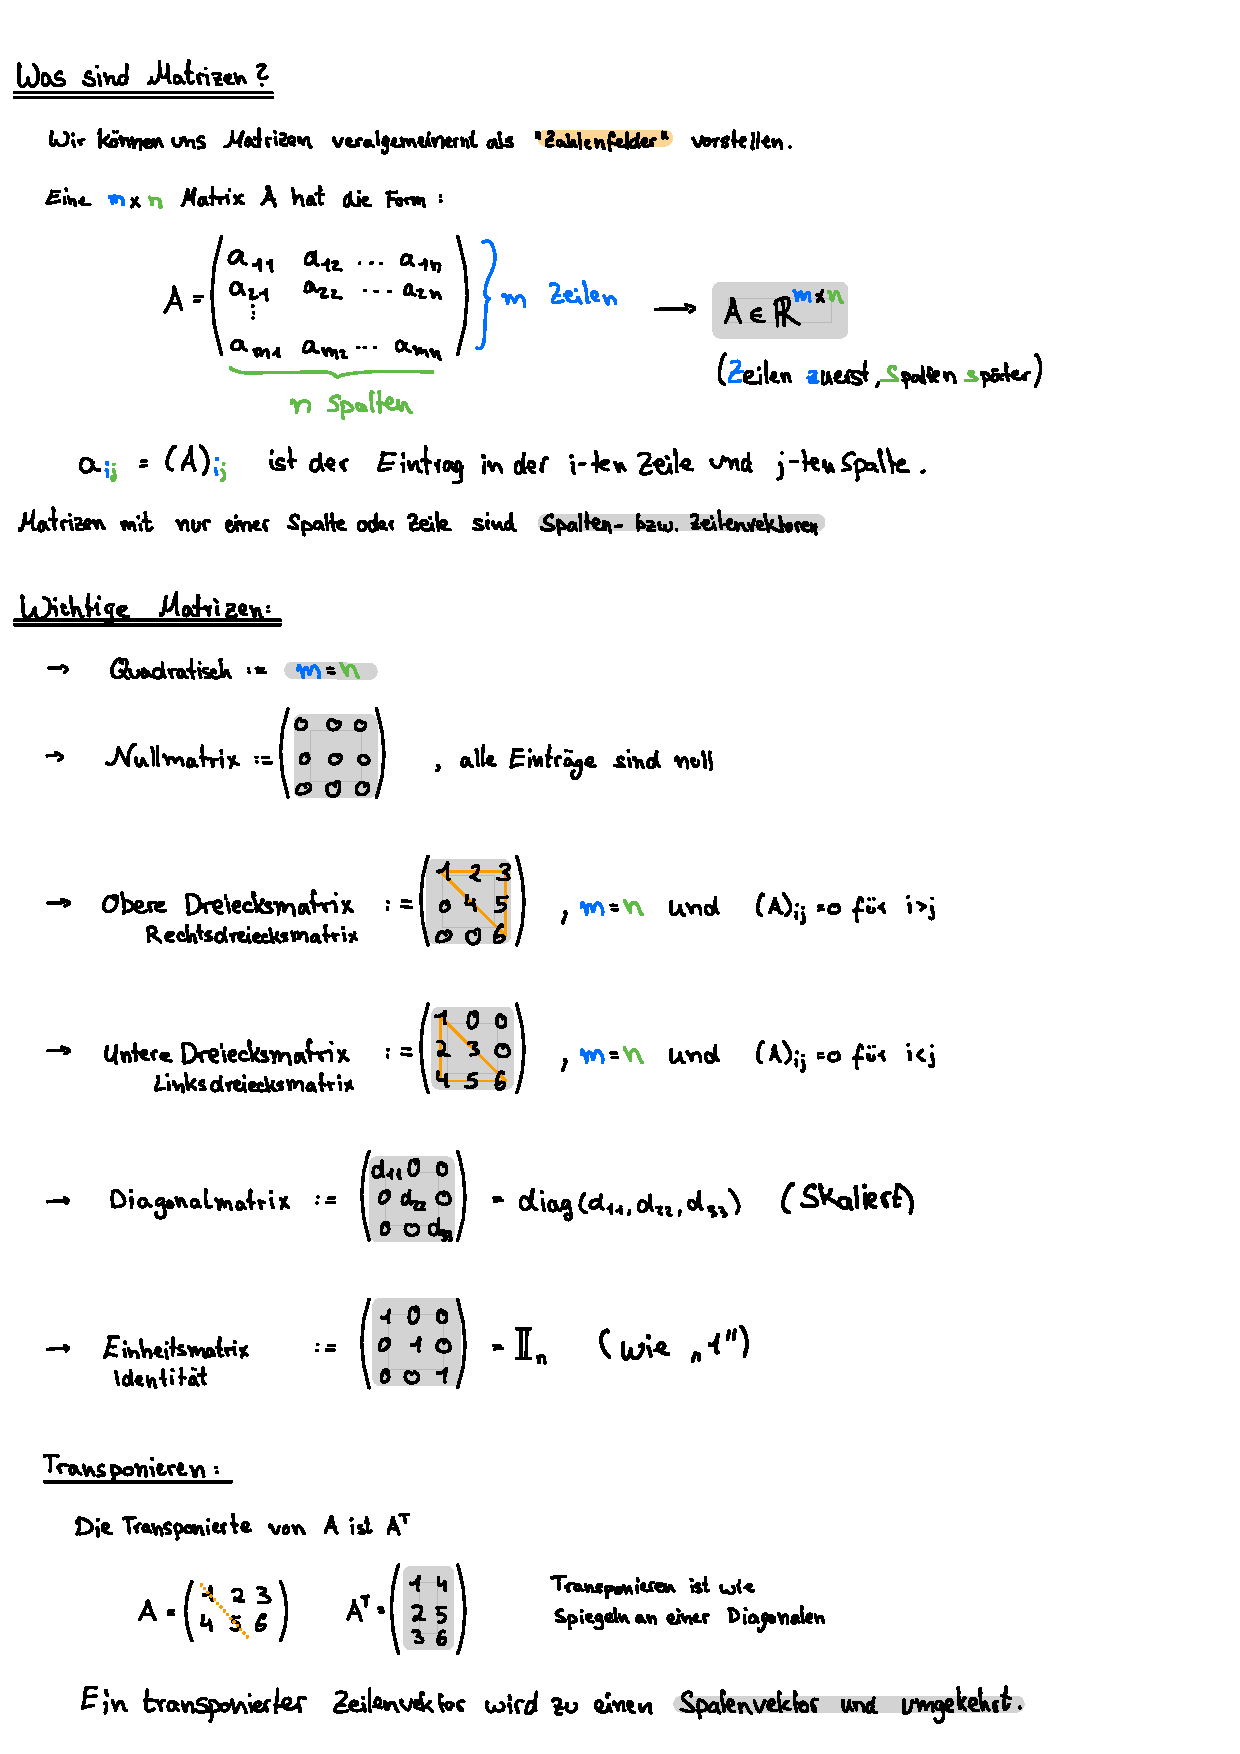
\includegraphics[page=1, scale=0.842]{pdf/02_Matrizen.pdf}
\end{figure}
\newpage
\includepdf[pages={2-}, 
            pagecommand={\thispagestyle{plain}}, 
            scale=0.95]{pdf/02_Matrizen.pdf}

\newgeometry{top=2.5cm, bottom=2cm}
\subsection{Beispielaufgaben} %Übung 06
\vspace{1cm}
\subsubsection{}
Was ist
\[
\begin{pmatrix}
0 & 0 & 1 & 0
\end{pmatrix}
\begin{pmatrix}
-1 & 1 & -1 & 2 \\
0 & 2 & 0 & -1 \\
-3 & 2 & -3 & 1 \\
2 & 1 & 2 & 3 \\
\end{pmatrix}
\begin{pmatrix}
-1 & 1 & -1 & 2 \\
0 & 2 & 0 & -1 \\
-3 & 2 & -3 & 1 \\
2 & 1 & 2 & 3 \\
\end{pmatrix}
\begin{pmatrix}
0\\
1\\
0\\
0\\
\end{pmatrix}?
\]

\textbf{Lösung:}

\newpage
\subsubsection{} %Adi PVK Tag 1
Für $a \in \mathbb{R}$  sei die Matrix
\[
A = \begin{pmatrix}
1 & 0 & 0 & 2 \\
0 & 1 & 0 & 0 \\
-1 & 0 & 1 & 0 \\
a & 1 & 0 & 1 \\
\end{pmatrix}
\]
gegeben. Für welche Werte von $a$ ist die Matrix $A$ singulär bzw. regulär? Bestimmen Sie für $a = 0$ die Inverse von $A$. \\

\noindent \textbf{Lösung:}

\newpage
\subsubsection{} %Zardini S.27
Bestimmen Sie die LR-Zerlegung der Matrix $A$, so dass $LR = PA$
\[
A = \begin{pmatrix}
0 & 1 & -3 \\
-3 & 7 & 6 \\
-3 & -2 & -2 \\
\end{pmatrix}.
\]

\textbf{Lösung:}
    \newgeometry{top=1cm, bottom=2cm}
\section{Determinante}
\begin{figure}[h!]
    \includegraphics[page=1, scale=0.842]{pdf/03_Determinante.pdf}
\end{figure}
\newpage
\includepdf[pages={2-}, 
            pagecommand={\thispagestyle{plain}}, 
            scale=0.95]{pdf/03_Determinante.pdf}

\newgeometry{top=2.5cm, bottom=2cm}
\subsection{Beispielaufgaben} 
\vspace{1cm}
\subsubsection{} % Zardini S. 36
Sei
\[
A = \begin{pmatrix}
1 & 4 & 8 \\
3 & 4 & 6 \\
2 & 1 & 1 \\
\end{pmatrix}
\]
Berechne $det(A^\top)$. \\

\noindent \textbf{Lösung:}
\vspace{6cm}

\subsubsection{}
Sei \[
A = \begin{pmatrix}
1 & 2 \\
3 & 4 \\
\end{pmatrix}
\]
Berechne $det(A^{-1})$. \\

\noindent \textbf{Lösung:}

\newpage
\subsubsection{} %Zardini S. 42
Seien $a, b, c, d \in \mathbb{R}$ und
\[
M = \begin{pmatrix}
a & 0 & 0 & 0 & 0 & 0 \\
1 & -2 & 0 & -1 & 0 & 0 \\
2 & b & 0 & 3 & 0 & 0 \\
0 & 7 & 1 & -2 & 0 & 0 \\
-1 & 4 & 0 & 7 & -1 & c \\
5 & 1 & d & 4 & 1 & 2 \\
\end{pmatrix}.
\]
\begin{enumerate}[label=\alph*)]
    \item Berechnen Sie $det(M)$
    \item Für welche $a, b, c, d$ ist $M$ singulär?
\end{enumerate}

\noindent \textbf{Lösung:}

\newpage
\subsubsection{}%Zardini S. 51
Seien $a, b, c, d \in \mathbb{R}$ und
\[
A = \begin{pmatrix}
a & b & c & d \\
-3a & 2b & 3c & 2d \\
a & b & -c & d \\
-2a & -2b & -2c & d \\
\end{pmatrix}.
\]
Berechnen Sie die Determinante von $A$. \\

\noindent \textbf{Lösung:}

\newpage
\subsubsection{}
Seien $a, b, c, d \in \mathbb{R}$ und
\[
A = \begin{pmatrix}
a & b & c & d & b & b & d \\
b & c & d & d & b & d & a \\
c & d & b & c & d & c & c \\
d & b & c & d & b & b & c \\
b & d & c & b & d & b & b \\
b & c & d & d & b & d & a \\
d & a & c & d & a & b & c \\
\end{pmatrix}.
\]
Berechnen Sie die Determinante von $A$. \\

\noindent \textbf{Lösung:}

    \newgeometry{top=1cm, bottom=2cm}
\section{Vektorräume}
\begin{figure}[h!]
    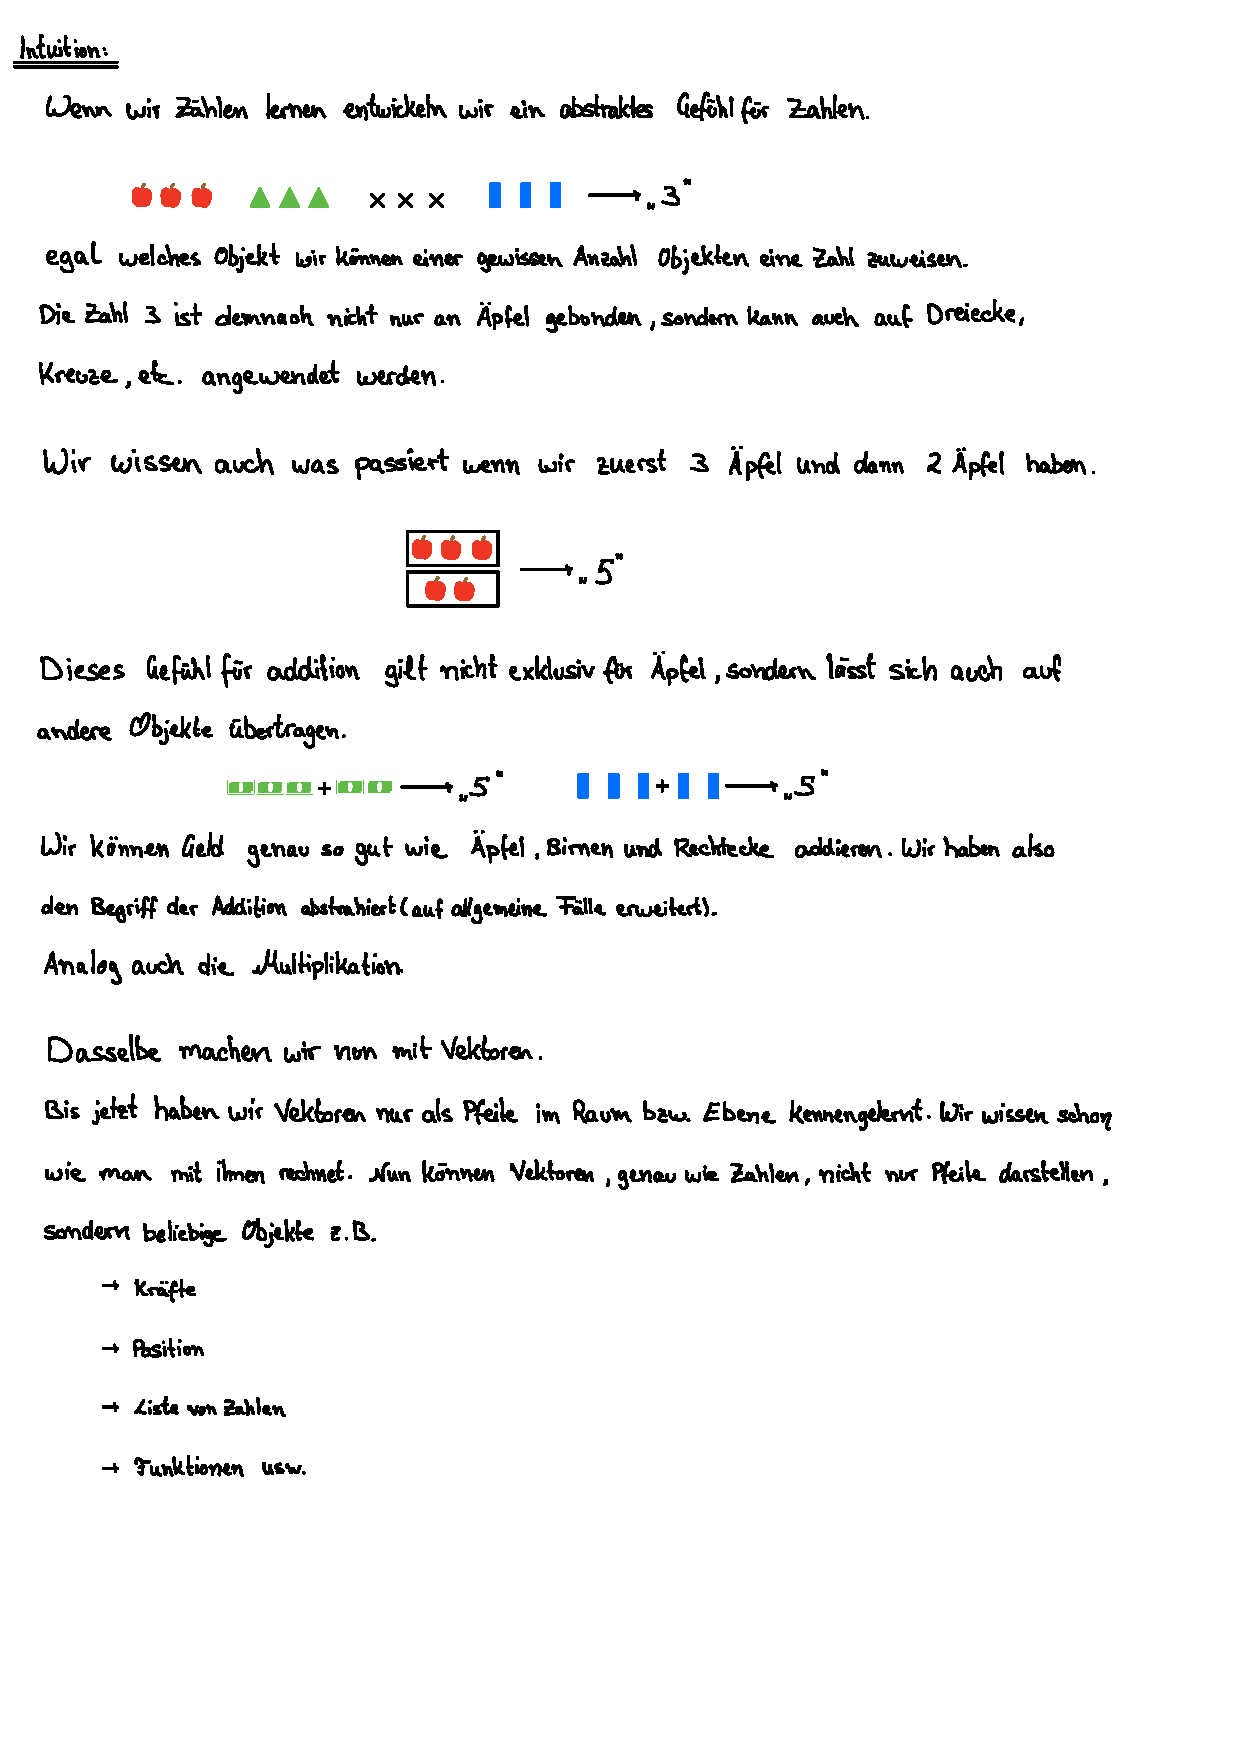
\includegraphics[page=1, scale=0.842]{pdf/04_Vektorraeume.pdf}
\end{figure}
\newpage
\includepdf[pages={2-}, 
            pagecommand={\thispagestyle{plain}}, 
            scale=0.95]{pdf/04_Vektorraeume.pdf}

\newgeometry{top=2.5cm, bottom=2cm}

\subsection{Beispielaufgaben} 

\vspace{1cm}

\subsubsection{} %Zardini S. 58
Seien

\begin{equation*}
    v_1 = 
    \begin{pmatrix}
    1\\
    0\\
    2\\
    \end{pmatrix}, v_2 =
    \begin{pmatrix}
    0\\
    1\\
    1\\
    \end{pmatrix}, v_3=
    \begin{pmatrix}
    0\\
    2\\
    2\\
    \end{pmatrix}, v_4=
    \begin{pmatrix}
    3\\
    0\\
    1\\
    \end{pmatrix}
\end{equation*}

Kann \( w = \begin{pmatrix} 4\\ 1\\ 2\\ \end{pmatrix} \) als eine Linearkombination von \( v_1,v_2,v_3,v_4 \) beschrieben werden? Falls ja, geben Sie eine Linearkombination an. 

\vspace{1\baselineskip}

\begin{solution}    

    \vspace{1\baselineskip}

    \leftskip=2em

    Dafür lösen wir folgendes LGS:

    \begin{equation*}
        \begin{gmatrix}[L]
            1 & 0 & 0 & 3 \\
            0 & 1 & 2 & 0 \\
            2 & 1 & 2 & 1
        \end{gmatrix} \hspace{-0.75em}
        \begin{gmatrix}[R]
            4 \\ 1 \\ 2
            \rowops
                \add[-2]{0}{2}
        \end{gmatrix} \rightarrow \; \begin{gmatrix}[L]
            1 & 0 & 0 & 3 \\
            0 & 1 & 2 & 0 \\
            0 & 1 & 2 & -5
        \end{gmatrix} \hspace{-0.75em}
        \begin{gmatrix}[R]
            4 \\ 1 \\ -6
                \rowops
                    \add[-1]{1}{2}
        \end{gmatrix} \rightarrow \; \begin{gmatrix}[L]
            1 & 0 & 0 & 3 \\
            0 & 1 & 2 & 0 \\
            0 & 0 & 0 & -5
        \end{gmatrix} \hspace{-0.75em}
        \begin{gmatrix}[R]
            4 \\ 1 \\ -7
        \end{gmatrix} 
    \end{equation*}

    \vspace{1\baselineskip}

    \begin{equation*}
        \left.
        \begin{aligned} 
            x_4 &= \frac{7}{5} \\
            x_3 &= t \\
            x_2 &= 1 - 2t \\
            x_1 &= 4 - 3\frac{7}{5} 
        \end{aligned} \;
        \right\} \; \xrightarrow{t=1} \begin{pmatrix}
            4 \\ 1 \\ 2
        \end{pmatrix} = - \frac{1}{5} \begin{pmatrix}
            1 \\ 0 \\ 2
        \end{pmatrix} - \begin{pmatrix}
            0 \\ 1 \\ 1
        \end{pmatrix} + \begin{pmatrix}
            0 \\ 2 \\ 2
        \end{pmatrix} + \frac{7}{5} \begin{pmatrix}
            3 \\ 0 \\ 1
        \end{pmatrix}.
    \end{equation*}

\end{solution}

\newpage

\subsubsection{} % Adi PVK Tag2

Es sei der Unterraum \( U \subset \mathbb{R}^3 \) gegeben durch 

\begin{equation*}
    U := \{(x,y,z)^\top \in \mathbb{R}^3:x+y+z=0\}
\end{equation*}

Bestimmen Sie eine Basis von \( U \). 

\vspace{1\baselineskip}

\begin{solution}    

    \leftskip=2em

    \begin{equation*}
        x = 0: \ v_1 = \begin{pmatrix}
            0 \\ 1 \\ -1
        \end{pmatrix}, \ y = 0: \ v_2 = \begin{pmatrix}
            1 \\ 0 \\ -1
        \end{pmatrix}, \ z = 0: \ v_3 = \begin{pmatrix}
            1 \\ -1 \\ 0
        \end{pmatrix}
    \end{equation*}

    aber \( v_3 = v_2 - v_1 \), also ist \( \{v_1,v_2\} \) bereits eine Basis von \( U \).

    \begin{equation*}
        \mathcal{B} = \left\{ \begin{pmatrix}
            0 \\ 1 \\ -1
        \end{pmatrix}, \begin{pmatrix}
            1 \\ 0 \\ -1
        \end{pmatrix} \right\}
    \end{equation*}

\end{solution}

\vspace{1cm}

\subsubsection{} %Übung 14

Überprüfen Sie, ob die folgenden Teilmengen Unterräume sind. Begründen Sie Ihre Antworten.
\begin{enumerate}[label=\alph*)]
    \item \( \mathbb{R}^3 \subset \mathbb{R}^3\).
    \item \( \{A\in \mathbb{C}^{n \times n}\: |\: A^\top = A \} \subset \mathbb{C}^{n \times n} \) für \( n \in \mathbb{N} \).
    \item  \( \{p \in \mathcal{P}_3\: |\: p(1) = 0 \) und  \( p(1100)=0\} \subset \mathcal{P}_3 \), wobei  \( \mathcal{P}_n \) für \( n \in \mathbb{N} \) der Vektorraum der Polynome mit Grad \( \leq n \) ist.
    \item \( \{(x_1, x_2, x_3)^\top \in \mathbb{R}^3 \: |\: \lvert x_1\rvert+\lvert x_2\rvert=\lvert x_3\rvert \}\subset \mathbb{R}^3 \)
\end{enumerate}

\vspace{1\baselineskip}

\begin{solution}    

    \vspace{1\baselineskip}

    \leftskip=2em

    \textbf{a)} 

    Enthält den Nullvektor: \( \begin{pmatrix} 0 \\ 0 \\ 0 \end{pmatrix} \in \mathbb{R}^3 \)

    \vspace{0.5\baselineskip}

    Abgeschlossen bez. Addition: \( \begin{pmatrix} x_1 \\ x_2 \\ x_3 \end{pmatrix} + \begin{pmatrix} y_1 \\ y_2 \\ y_3 \end{pmatrix} = \begin{pmatrix} x_1 + y_1 \\ x_2 + y_2 \\ x_3 + y_3 \end{pmatrix} \in \mathbb{R}^3, \ \forall x_i, y_i \in \mathbb{R} \)

    \vspace{0.5\baselineskip}

    Abgeschlossen bez. Multiplikation: \( \alpha \cdot \begin{pmatrix}
        x_1 \\ x_2 \\ x_3
    \end{pmatrix} \in \mathbb{R}^3 \ \forall \alpha \in \mathbb{R} \)

    \( \mathbb{R}^3 \subset \mathbb{R}^3 \) ist ein Unterraum.

    \vspace{4\baselineskip}

    \textbf{b)} 

    Enthält den Nullvektor: \( \begin{pmatrix}
        0 & 0 \\
        0 & 0
    \end{pmatrix}^\top = \begin{pmatrix}
        0 & 0 \\
        0 & 0
    \end{pmatrix} \)

    \vspace{0.5\baselineskip}

    Abgeschlossen bez. Addition: 
    \begin{equation*}
        \begin{pmatrix}
            a_{11} & \textcolor{red}{a_{21}} \\
            \textcolor{red}{a_{21}} & a_{22}
        \end{pmatrix} + \begin{pmatrix}
            b_{11} & \textcolor{red}{b_{21}} \\
            \textcolor{red}{b_{21}} & b_{22}
        \end{pmatrix} = \begin{pmatrix}
            a_{11} + b_{11} & \textcolor{red}{a_{21} + b_{21}} \\
            \textcolor{red}{a_{21} + b_{21}} & a_{22} + b_{22}
            \end{pmatrix}^\top = \begin{pmatrix}
            a_{11} + b_{11} & \textcolor{red}{a_{21} + b_{21}} \\
            \textcolor{red}{a_{21} + b_{21}} & a_{22} + b_{22}
        \end{pmatrix}
    \end{equation*}

    Abgeschlossen bez. Multiplikation: \( \alpha \cdot \begin{pmatrix}
        a_{11} & \textcolor{red}{a_{21}} \\
        \textcolor{red}{a_{21}} & a_{22}
    \end{pmatrix} = \alpha \cdot \begin{pmatrix}
        a_{11} & \textcolor{red}{a_{21}} \\
        \textcolor{red}{a_{21}} & a_{22}
    \end{pmatrix}^\top \ \forall \alpha \in \mathbb{R} \)

    \vspace{1\baselineskip}

    \( \{A\in \mathbb{C}^{n \times n}\: |\: A^\top = A \} \subset \mathbb{C}^{n \times n} \) ist ein Unterraum.

    \vspace{1\baselineskip}

    \textbf{c)}

    \vspace{0.5\baselineskip}

    Enthält den Nullvektor: \( p_0(x) = 0x^3 + 0x^2 + 0x + 0. \)

    \begin{equation*}
        p_0(1) = 0 \quad \text{und} \quad p_0(1100) = 0.
    \end{equation*}

    \vspace{0.5\baselineskip}

    Abgeschlossen bez. Addition:    

    \begin{figure}[h]
        \centering
        \tikzset{every picture/.style={line width=0.75pt}} %set default line width to 0.75pt        
        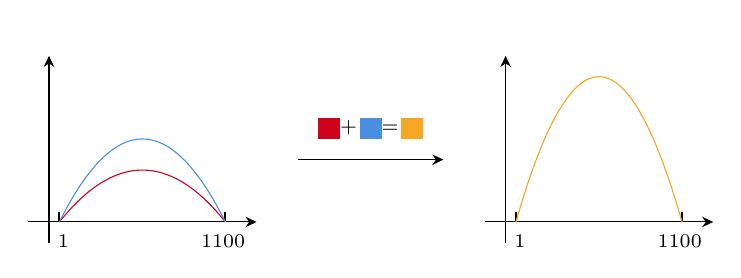
\begin{tikzpicture}[x=0.75pt,y=0.75pt,yscale=-1,xscale=1]
            %uncomment if require: \path (0,300); %set diagram left start at 0, and has height of 300

            %Straight Lines [id:da34248100016212457] 
            \draw    (170,90) -- (277,90) ;
            \draw [shift={(280,90)}, rotate = 180] [fill={rgb, 255:red, 0; green, 0; blue, 0 }  ][line width=0.08]  [draw opacity=0] (5.36,-2.57) -- (0,0) -- (5.36,2.57) -- (3.56,0) -- cycle    ;
            %Straight Lines [id:da8980030736411168] 
            \draw    (180,100) -- (180,13) ;
            \draw [shift={(180,10)}, rotate = 90] [fill={rgb, 255:red, 0; green, 0; blue, 0 }  ][line width=0.08]  [draw opacity=0] (5.36,-2.57) -- (0,0) -- (5.36,2.57) -- (3.56,0) -- cycle    ;
            %Straight Lines [id:da8756913546199198] 
            \draw [line width=0.75]    (185,85) -- (185,90) ;
            %Straight Lines [id:da1320233507901698] 
            \draw [line width=0.75]    (265,85) -- (265,90) ;
            %Shape: Parabola [id:dp8938018456449416] 
            \draw  [color={rgb, 255:red, 208; green, 2; blue, 27 }  ,draw opacity=1 ] (265,90) .. controls (238.33,56.67) and (211.67,56.67) .. (185,90) ;
            %Shape: Parabola [id:dp7154214398607968] 
            \draw  [color={rgb, 255:red, 74; green, 144; blue, 226 }  ,draw opacity=1 ] (265,90) .. controls (238.33,36.67) and (211.67,36.67) .. (185,90) ;
            %Straight Lines [id:da6661026753051024] 
            \draw    (390,90) -- (497,90) ;
            \draw [shift={(500,90)}, rotate = 180] [fill={rgb, 255:red, 0; green, 0; blue, 0 }  ][line width=0.08]  [draw opacity=0] (5.36,-2.57) -- (0,0) -- (5.36,2.57) -- (3.56,0) -- cycle    ;
            %Straight Lines [id:da5432422995538024] 
            \draw    (400,100) -- (400,13) ;
            \draw [shift={(400,10)}, rotate = 90] [fill={rgb, 255:red, 0; green, 0; blue, 0 }  ][line width=0.08]  [draw opacity=0] (5.36,-2.57) -- (0,0) -- (5.36,2.57) -- (3.56,0) -- cycle    ;
            %Straight Lines [id:da9027214096380924] 
            \draw [line width=0.75]    (405,85) -- (405,90) ;
            %Straight Lines [id:da6657825405781942] 
            \draw [line width=0.75]    (485,85) -- (485,90) ;
            %Shape: Parabola [id:dp0673950229164001] 
            \draw  [color={rgb, 255:red, 245; green, 166; blue, 35 }  ,draw opacity=1 ] (485,90) .. controls (458.33,-3.33) and (431.67,-3.33) .. (405,90) ;
            %Straight Lines [id:da6162418070851343] 
            \draw    (300,60) -- (367,60) ;
            \draw [shift={(370,60)}, rotate = 180] [fill={rgb, 255:red, 0; green, 0; blue, 0 }  ][line width=0.08]  [draw opacity=0] (5.36,-2.57) -- (0,0) -- (5.36,2.57) -- (3.56,0) -- cycle    ;
            %Shape: Rectangle [id:dp379274645803359] 
            \draw  [color={rgb, 255:red, 208; green, 2; blue, 27 }  ,draw opacity=1 ][fill={rgb, 255:red, 208; green, 2; blue, 27 }  ,fill opacity=1 ] (310,40) -- (320,40) -- (320,50) -- (310,50) -- cycle ;
            %Shape: Rectangle [id:dp8222817282747726] 
            \draw  [color={rgb, 255:red, 74; green, 144; blue, 226 }  ,draw opacity=1 ][fill={rgb, 255:red, 74; green, 144; blue, 226 }  ,fill opacity=1 ] (330,40) -- (340,40) -- (340,50) -- (330,50) -- cycle ;
            %Shape: Rectangle [id:dp557713999550064] 
            \draw  [color={rgb, 255:red, 245; green, 166; blue, 35 }  ,draw opacity=1 ][fill={rgb, 255:red, 245; green, 166; blue, 35 }  ,fill opacity=1 ] (350,40) -- (360,40) -- (360,50) -- (350,50) -- cycle ;

            % Text Node
            \draw (183,95) node [anchor=north west][inner sep=0.75pt]  [font=\scriptsize] [align=left] {$\displaystyle 1$};
            % Text Node
            \draw (252,95) node [anchor=north west][inner sep=0.75pt]  [font=\scriptsize] [align=left] {$\displaystyle 1100$};
            % Text Node
            \draw (403,95) node [anchor=north west][inner sep=0.75pt]  [font=\scriptsize] [align=left] {$\displaystyle 1$};
            % Text Node
            \draw (472,95) node [anchor=north west][inner sep=0.75pt]  [font=\scriptsize] [align=left] {$\displaystyle 1100$};
            % Text Node
            \draw (319,40) node [anchor=north west][inner sep=0.75pt]  [font=\scriptsize] [align=left] {$\displaystyle +$};
            % Text Node
            \draw (339,42) node [anchor=north west][inner sep=0.75pt]  [font=\scriptsize] [align=left] {=};
        \end{tikzpicture}
    \end{figure}

    Abgeschlossen bez. Multiplikation:

    \begin{figure}[h]
        \centering
        \tikzset{every picture/.style={line width=0.75pt}} %set default line width to 0.75pt        
        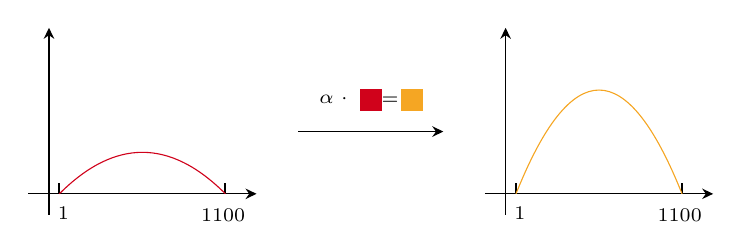
\begin{tikzpicture}[x=0.75pt,y=0.75pt,yscale=-1,xscale=1]
            %uncomment if require: \path (0,300); %set diagram left start at 0, and has height of 300

            %Straight Lines [id:da34248100016212457] 
            \draw    (170,90) -- (277,90) ;
            \draw [shift={(280,90)}, rotate = 180] [fill={rgb, 255:red, 0; green, 0; blue, 0 }  ][line width=0.08]  [draw opacity=0] (5.36,-2.57) -- (0,0) -- (5.36,2.57) -- (3.56,0) -- cycle    ;
            %Straight Lines [id:da8980030736411168] 
            \draw    (180,100) -- (180,13) ;
            \draw [shift={(180,10)}, rotate = 90] [fill={rgb, 255:red, 0; green, 0; blue, 0 }  ][line width=0.08]  [draw opacity=0] (5.36,-2.57) -- (0,0) -- (5.36,2.57) -- (3.56,0) -- cycle    ;
            %Straight Lines [id:da8756913546199198] 
            \draw [line width=0.75]    (185,85) -- (185,90) ;
            %Straight Lines [id:da1320233507901698] 
            \draw [line width=0.75]    (265,85) -- (265,90) ;
            %Shape: Parabola [id:dp8938018456449416] 
            \draw  [color={rgb, 255:red, 208; green, 2; blue, 27 }  ,draw opacity=1 ] (265,90) .. controls (238.33,63.33) and (211.67,63.33) .. (185,90) ;
            %Straight Lines [id:da6661026753051024] 
            \draw    (390,90) -- (497,90) ;
            \draw [shift={(500,90)}, rotate = 180] [fill={rgb, 255:red, 0; green, 0; blue, 0 }  ][line width=0.08]  [draw opacity=0] (5.36,-2.57) -- (0,0) -- (5.36,2.57) -- (3.56,0) -- cycle    ;
            %Straight Lines [id:da5432422995538024] 
            \draw    (400,100) -- (400,13) ;
            \draw [shift={(400,10)}, rotate = 90] [fill={rgb, 255:red, 0; green, 0; blue, 0 }  ][line width=0.08]  [draw opacity=0] (5.36,-2.57) -- (0,0) -- (5.36,2.57) -- (3.56,0) -- cycle    ;
            %Straight Lines [id:da9027214096380924] 
            \draw [line width=0.75]    (405,85) -- (405,90) ;
            %Straight Lines [id:da6657825405781942] 
            \draw [line width=0.75]    (485,85) -- (485,90) ;
            %Shape: Parabola [id:dp0673950229164001] 
            \draw  [color={rgb, 255:red, 245; green, 166; blue, 35 }  ,draw opacity=1 ] (485,90) .. controls (458.33,23.33) and (431.67,23.33) .. (405,90) ;
            %Straight Lines [id:da6162418070851343] 
            \draw    (300,60) -- (367,60) ;
            \draw [shift={(370,60)}, rotate = 180] [fill={rgb, 255:red, 0; green, 0; blue, 0 }  ][line width=0.08]  [draw opacity=0] (5.36,-2.57) -- (0,0) -- (5.36,2.57) -- (3.56,0) -- cycle    ;
            %Shape: Rectangle [id:dp379274645803359] 
            \draw  [color={rgb, 255:red, 208; green, 2; blue, 27 }  ,draw opacity=1 ][fill={rgb, 255:red, 208; green, 2; blue, 27 }  ,fill opacity=1 ] (330,40) -- (340,40) -- (340,50) -- (330,50) -- cycle ;
            %Shape: Rectangle [id:dp557713999550064] 
            \draw  [color={rgb, 255:red, 245; green, 166; blue, 35 }  ,draw opacity=1 ][fill={rgb, 255:red, 245; green, 166; blue, 35 }  ,fill opacity=1 ] (350,40) -- (360,40) -- (360,50) -- (350,50) -- cycle ;

            % Text Node
            \draw (183,95) node [anchor=north west][inner sep=0.75pt]  [font=\scriptsize] [align=left] {$\displaystyle 1$};
            % Text Node
            \draw (252,96) node [anchor=north west][inner sep=0.75pt]  [font=\scriptsize] [align=left] {$\displaystyle 1100$};
            % Text Node
            \draw (403,95) node [anchor=north west][inner sep=0.75pt]  [font=\scriptsize] [align=left] {$\displaystyle 1$};
            % Text Node
            \draw (472,96) node [anchor=north west][inner sep=0.75pt]  [font=\scriptsize] [align=left] {$\displaystyle 1100$};
            % Text Node
            \draw (339,42) node [anchor=north west][inner sep=0.75pt]  [font=\scriptsize] [align=left] {=};
            % Text Node
            \draw (309,41) node [anchor=north west][inner sep=0.75pt]  [font=\scriptsize] [align=left] {$\displaystyle \alpha \ \cdotp $};
        \end{tikzpicture}
    \end{figure}

    \( \{p \in \mathcal{P}_3\: |\: p(1) = 0 \) und  \( p(1100)=0\} \subset \mathcal{P}_3 \) ist ein Unterraum.

    \vspace{1\baselineskip}

    \textbf{d)}

    Enthält den Nullvektor: \( |0| + |0| = |0| \)

    \vspace{0.5\baselineskip}

    Abgeschlossen bez. Addition:

    \begin{equation*}
        \begin{pmatrix}
            1 \\ 0 \\ 1
        \end{pmatrix} + \begin{pmatrix}
            0 \\ -1 \\ -1
        \end{pmatrix} = \begin{pmatrix}
            1 \\ -1 \\ 0
        \end{pmatrix} \quad \Rightarrow \quad |1| + |-1| = |2| \neq |0|
    \end{equation*}

    Nicht abgeschlossen bez. Addition, also kein Unterraum.

\end{solution}

\newpage

\subsubsection{} %Adi PVK Tag 2

Betrachten Sie den Vektorraum \( \mathcal{P}_3 \) der reellen Polynome vom Grad \( \leq \) 3 mit der Basis \( \mathcal{B} = \{x^3+1,x^2+x-2,2x+1,x+2\} \).

\begin{enumerate}[label=\alph*)]
    \item Welches Polynom in \( \mathcal{P}_3 \) hat die Koordinaten \( (2,1,-1,3)^\top \) bezüglich \( \mathcal{B} \)?
    \item Sei \( p(x):=x^3+x^2+x+1 \). Bestimmen Sie die Koordinaten von \( p(x) \) bezüglich \( \mathcal{B} \).
\end{enumerate}

\vspace{1\baselineskip}

\begin{solution}    

    \vspace{1\baselineskip}

    \leftskip=2em

    \textbf{a)}

    \begin{equation*}
        \begin{aligned}
            p(x) &= 2(x^3+1) + 1(x^2+x-2) - 1(2x+1) + 3(x+2) \\
            &= 2x^3 + 2 + x^2 + x - 2 - 2x - 1 + 3x + 6 \\            
            &= 2x^3 + x^2 + 2x + 5.
        \end{aligned}
    \end{equation*}

    \textbf{b)}

    \begin{equation*}
        \begin{gmatrix}[L]
            1 & 0 & 0 & 0 \\
            0 & 1 & 0 & 0 \\
            0 & 1 & 2 & 1 \\
            1 & -2 & 1 & 2
        \end{gmatrix} \hspace{-0.75em} \begin{gmatrix}[R]
            1 \\ 1 \\ 1 \\ 1
            \rowops
                \add[-1]{0}{3}
        \end{gmatrix} \rightarrow \; \begin{gmatrix}[L]
            1 & 0 & 0 & 0 \\
            0 & 1 & 0 & 0 \\
            0 & 1 & 2 & 1 \\
            0 & -2 & 1 & 2
        \end{gmatrix} \hspace{-0.75em} \begin{gmatrix}[R]
            1 \\ 1 \\ 1 \\ 0
            \rowops
                \add[-1]{1}{2}
                \add[2]{1}{3}
        \end{gmatrix} \hspace{-0.75em} \rightarrow \; \begin{gmatrix}[L]
            1 & 0 & 0 & 0 \\
            0 & 1 & 0 & 0 \\
            0 & 0 & 2 & 1 \\
            0 & 0 & 1 & 2
        \end{gmatrix} \hspace{-0.75em} \begin{gmatrix}[R]
            1 \\ 1 \\ 0 \\ 2
            \rowops
                \swap{2}{3}
            \end{gmatrix} 
    \end{equation*}

    \vspace{0.5\baselineskip}

    \begin{equation*}
        \rightarrow \;
        \begin{gmatrix}[L]
            1 & 0 & 0 & 0 \\
            0 & 1 & 0 & 0 \\
            0 & 0 & 1 & 2 \\
            0 & 0 & 2 & 1
        \end{gmatrix} \hspace{-0.75em} \begin{gmatrix}[R]
            1 \\ 1 \\ 2 \\ 0
            \rowops
                \add[-2]{2}{3}
        \end{gmatrix} \rightarrow \; \begin{gmatrix}[L]
            1 & 0 & 0 & 0 \\
            0 & 1 & 0 & 0 \\
            0 & 0 & 1 & 2 \\
            0 & 0 & 0 & -3
        \end{gmatrix} \hspace{-0.75em} \begin{gmatrix}[R]
            1 \\ 1 \\ 2 \\ -4
        \end{gmatrix} \rightarrow \quad \begin{aligned}
            x_4 &= \frac{4}{3} \\
            x_3 &= - \frac{2}{3} \\
            x_2 &= 1 \\
            x_1 &= 1
        \end{aligned}
    \end{equation*}

    Die Koordinaten von \( p(x) \) bezüglich \( \mathcal{B} \) sind also

    \begin{equation*}
        [p(x)]_{\mathcal{B}} = \begin{pmatrix}
            1 \\ 1 \\ -\frac{2}{3} \\ \frac{4}{3}
        \end{pmatrix}.
    \end{equation*}

\end{solution}

\newpage

\subsubsection{} %Prüfung S12

Sei \( V \) der von den Funktionen \( \{1,x,x^2,e^x\} \) aufgespannte Vektorraum mit dem Unterraum \( U:=\{1,x,x^2\} \). Für zwei Funktionen \( f,g \in V \) sei das folgende Skalarprodukt definiert:

\begin{equation*}
    \langle f,g \rangle := f(0)g(0)+f'(0)g'(0)+f''(0)g''(0)+f'''(0)g'''(0).
\end{equation*}

\begin{enumerate}[label=\alph*)]
    \item Wie lautet die Norm von \( f \in V \) bezüglich des gegebenen Skalarprodukts?
    \item Bestimmen Sie eine Orthonormalbasis in \( U \) bezüglich des gegebenen Skalarprodukts.
    \item Verifizieren Sie, dass \( \langle . \:,. \rangle \) tatsächlich ein Skalarprodukt ist.
\end{enumerate}

\vspace{1\baselineskip}

\begin{solution}    

    \vspace{1\baselineskip}

    \leftskip=2em

    \textbf{a)} \( \qquad ||f|| = \sqrt{f(0)^2 + f'(0)^2 + f''(0)^2 + f'''(0)^2} \)

    \vspace{1.5\baselineskip}

    \textbf{b)} Gram-Schmidt: \( b_1 = 1, \ b_2 = x, \ b_3 = x^2 \)

    \begin{equation*}
        \begin{aligned}
            \rightarrow \ e_1 &= \frac{1}{||1||} \qquad \qquad \rightarrow e_2' = b_2 - \underbrace{\langle b_2,e_1 \rangle}_{=0} e_1 = x \\
            & \hspace{3.65cm} e_2 = \frac{e_2'}{||e_2'||} = x \\[1.75em]
            \rightarrow e_3' &= b_3 - \underbrace{\langle b_3,e_2 \rangle}_{=0} e_2 - \underbrace{\langle b_3,e_1 \rangle}_{=0} e_1 = x^2 \\
            \qquad e_3 &= \frac{e_3'}{||e_3'||} = \frac{x^2}{2} \hspace{5cm} \mathcal{B} = \left\{ 1, x, \frac{x^2}{2} \right\}
        \end{aligned}
    \end{equation*}

    \vspace{1\baselineskip}

    \textbf{c)} \( \quad x, y, z \in V \)
    
    \begin{equation*}
        \begin{aligned}
            \textcolor{red}{\langle x, y+z \rangle} &= x(0)[y(0)+z(0)] + x'(0)[y'(0)+z'(0)] + x''(0)[y''(0)+z''(0)] \\ 
            & \quad + x'''(0)[y'''(0)+z'''(0)] \\
            &= x(0)y(0) + x(0)z(0) + x'(0)y'(0) + x'(0)z'(0) + x''(0)y''(0) \\
            & \quad + x''(0)z''(0) + x'''(0)y'''(0) + x'''(0)z'''(0) = \textcolor{red}{\langle x,y \rangle + \langle x,z \rangle}. \\[0.5em]
            \textcolor{red}{\langle x, \alpha y \rangle} &= x(0)(\alpha y(0)) + x'(0)(\alpha y'(0)) + x''(0)(\alpha y''(0)) + x'''(0)(\alpha y'''(0)) \\
            &= \alpha \left[ x(0)y(0) + x'(0)y'(0) + x''(0)y''(0) + x'''(0)y'''(0) \right] = \textcolor{red}{\alpha \langle x,y \rangle}. \\[0.5em]
            \textcolor{red}{\langle x, y \rangle} &= x(0)y(0) + x'(0)y'(0) + x''(0)y''(0) + x'''(0)y'''(0) = \textcolor{red}{\langle y, x \rangle}. \\[0.5em]
            \textcolor{red}{\langle x, x \rangle} &= x(0)^2 + x'(0)^2 + x''(0)^2 + x'''(0)^2 \ \textcolor{red}{\geq 0}. \\[0.5em]
            \textcolor{red}{\langle f, f \rangle} &= 0 \; \Leftrightarrow \; \textcolor{red}{f \equiv 0}, \ e^x-\text{Term sonst nie Null}. 
        \end{aligned}
    \end{equation*}


\end{solution}

\newpage

\subsubsection{} %Zardini S.70

Sei folgendes Skalarprodukt auf \( \mathcal{P}_4 \) gegeben

\begin{equation*}
    \langle p,q \rangle = \int_{0}^{1} p(x)q(x) \,dx.
\end{equation*}

Finden Sie eine Orthonormalbasis für den Vektorraum span\( \{1,3x^4\} \). 

\vspace{1\baselineskip}

\begin{solution}    

    \vspace{1\baselineskip}

    \leftskip=2em

    Gram-Schmidt: \( b_1 = 1, \ b_2 = 3x^4 \)

    \begin{equation*}
        \begin{aligned}
            \rightarrow e_1 &= \frac{b_1}{||b_1||} = 1 \\[2em]
            \rightarrow e_2' &= b_2 - \underbrace{\langle b_2,e_1 \rangle} e_1 \\
            & \hspace{1.65cm} \int_{0}^{1} 3x^4 dx = \frac{3}{5} \\[0.5em]
            e_2' &= 3x^4 - \frac{3}{5} \\[1.5em]
            e_2 &= \frac{e_2'}{||e_2'||} \\
            & \hspace{0.6cm} ||e_2'|| = \sqrt{\int_{0}^{1} (3x^4 - \frac{3}{5})^2 dx} = \frac{4}{5} \\[0.5em]
            e_2 &= \frac{5}{4} (3x^4 - \frac{3}{5}) = \frac{3}{4}(5x^4 - 1)
        \end{aligned}
    \end{equation*}

    \vspace{1\baselineskip}

    Eine Orthonormalbasis ist dann gegeben durch

    \begin{equation*}
        \mathcal{B} = \left\{ 1, \frac{3}{4}(5x^4 - 1) \right\}.
    \end{equation*}

\end{solution}

    \newgeometry{top=1cm, bottom=2cm}
\section{Lineare Abbildungen}
\begin{figure}[h!]
    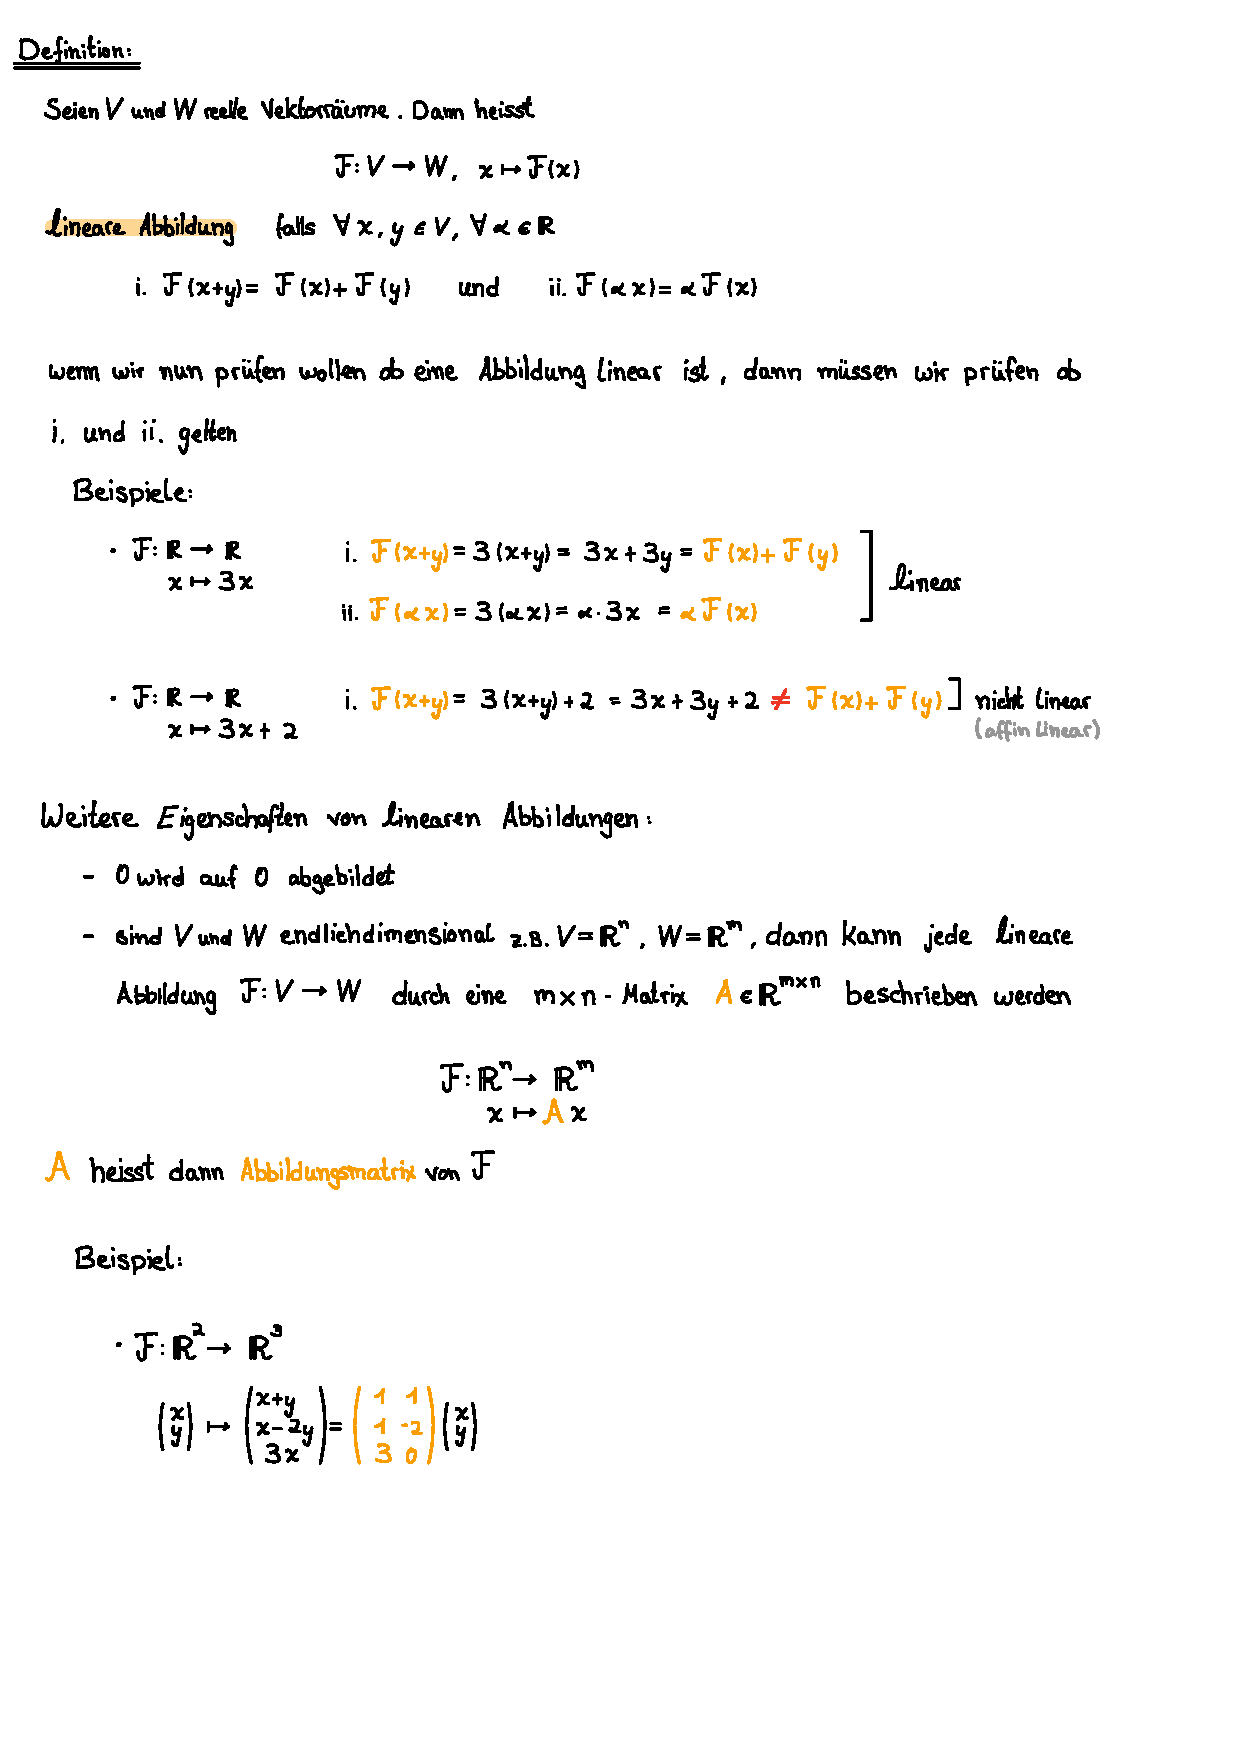
\includegraphics[page=1, scale=0.842]{pdf/05_Lineare_Abbildungen.pdf}
\end{figure}
\newpage
\includepdf[pages={2-}, 
            pagecommand={\thispagestyle{plain}}, 
            scale=0.95]{pdf/05_Lineare_Abbildungen.pdf}

\newgeometry{top=2.5cm, bottom=2cm}
\subsection{Beispielaufgaben} %Übung 01
\vspace{1cm}
\subsubsection{} %serie 06
Sei
\[
A = \begin{pmatrix}
2 & 1 & -1 & 2 \\
1 & 0 & -1 & 0 \\
3 & 1 & -2 & 2 \\
\end{pmatrix}.
\]
Bestimmen Sie eine Basis für das Bild und den Kern von $A$. \\

\noindent \textbf{Lösung:}
\vspace{5cm}

\subsubsection{} %Prüfiung S.12
Sei $\mathcal{P}_2$ der Vektorraum der Polynome vom Grad $\leq 2$ mit der Basis $\mathcal{B} = \{1,x,x^2\}$. Sei
\[\begin{aligned}
\mathcal{L}: \; \mathcal{P}_2 &\rightarrow \mathcal{P}_2 \\
p(x) &\mapsto p''(x)+4p'(x)+3p(x)
\end{aligned}\] \\
Bestimmen Sie die Darstellungsmatrix von $\mathcal{L}$ bezüglich der Basis $\mathcal{B}$.\\

\noindent \textbf{Lösung:}

\newpage
\subsubsection{}
Geben seinen die Abbildungen
\begin{enumerate}[label=\alph*)]
    \item $\mathcal{F}: \mathbb{R}^2 \rightarrow \mathbb{R}^2,\; (x_1,x_2)^\top \mapsto (2x_1+x_2,x_1)^\top $
    \item $\mathcal{G}: \mathcal{C} ([x_0,x_1], \mathbb{R}) \rightarrow \mathbb{R},\; g(x) \mapsto \int_{x_0}^{x_1} g(x) \,dx$
\end{enumerate}
Prüfe ob die Abbildungen $\mathcal{F,G}$ linear sind.\\

\noindent \textit{Tipp}: $\mathcal{C} ([x_0,x_1], \mathbb{R})$ beschreibt alle stetigen Funktionen auf dem Intervall $[x_0,x_1]$. \\

\noindent \textbf{Lösung:}

% \newpage
% \subsubsection{}
% Sei $V = \mathcal{P}_2$ und $W = \mathcal{P}_1$. Wobei V durch die Basis $\mathcal{B} = (1,x,x^2)$ und $W$ durch die Basis $\mathcal{C} = (1,x)$ beschrieben werden kann. sei ausserdem
% \[\begin{aligned}
% \mathcal{F}: \; V &\rightarrow W \\
% p(x) &\mapsto p'(x)+p''(x)
% \end{aligned}\]
% Bestimme die Abbildungsmatrix $A$ der Abbildung $\mathcal{F}$. \\

% \noindent \textbf{Lösung:}

\newpage
\subsubsection{} %Serie 06
Gegeben Sei der Vektorraum $V = \mathbb{R}^3$ mit der Standardbasis $\mathcal{B}$. Die Matrix
\[
A = \begin{pmatrix}
-\frac{5}{6} & \frac{1}{6} & \frac{1}{3} \\
\frac{1}{6}  & -\frac{5}{6} & \frac{1}{3} \\
\frac{1}{3} & \frac{1}{3} & -\frac{1}{3} \\
\end{pmatrix}.
\]
definiert eine lineare Abbildung von $V$ nach $V$.
\begin{enumerate}[label=\alph*)]
    \item Durch eine Wahl der neuen Basis
           \[ \mathcal{B}' = \Biggl\{ 
                                \begin{pmatrix}
                                2\\
                                0\\
                                -1\\
                                \end{pmatrix},
                                \begin{pmatrix}
                                -1\\
                                1\\
                                0\\
                                \end{pmatrix},
                                \begin{pmatrix}
                                1\\
                                1\\
                                2\\
                                \end{pmatrix}
                                \Biggr\}.
                                \]
            werden neue Koordianten eingeführt. Bestimmen Sie die Übergangsmatrix $T$ von $\mathcal{B}$ nach $\mathcal{B}'$.
            \item Durch welche Matrix $B$ wird die lineare Abbildung in den neuen Koordinaten $\mathcal{B}'$ beschrieben?
\end{enumerate}

\newpage
\subsubsection{} %Zardini S.84
Betrachten Sie die Abbildung $\mathcal{F}: \mathbb{R}^3 \rightarrow \mathbb{R}^3$ gegeben durch
\[
\begin{pmatrix}
x\\
y\\
z\\
\end{pmatrix} \mapsto
\begin{pmatrix}
7x+5y-8z\\
5x+3y-4z\\
-x-3y+8z\\
\end{pmatrix}
\]
\begin{enumerate}[label=\alph*)]
    \item Geben Sie die Darstellungsmatrix von $\mathcal{F}$ bezüglich der Standardbasis $\mathcal{E} = \{e_1,e_2,e_3\}$ von $\mathbb{R}^3$ an.
    \item Gegeben sei die Basis $\mathcal{B} = \{b_1 := e_1,\; b_2 :=e_1+e_2,\; b_3 := e_2+e_3 \}$ von $\mathbb{R}^3$. Finden Sie die Übergangsmatrix $T$ von $\mathcal{B}$ nach $\mathcal{E}$ und ihre Inverse $T^{-1}$.
    \item Berechnen Sie die Darstellungsmatrix von $\mathcal{F}$ bezüglich $\mathcal{B}$ unter Verwendung der Übergangsmatrix $T$ und ihrer Inversen.
    \item Bestimmen Sie eine Basis des Kerns von $\mathcal{F}$ und eine Basis des Bildes von $\mathcal{F}$. Geben Sie ausserdem die jeweiligen Dimensionen an.
\end{enumerate}

\noindent \textbf{Lösung:}
    \newgeometry{top=1cm, bottom=2cm}
\section{Eigenwertproblem}
\begin{figure}[h!]
    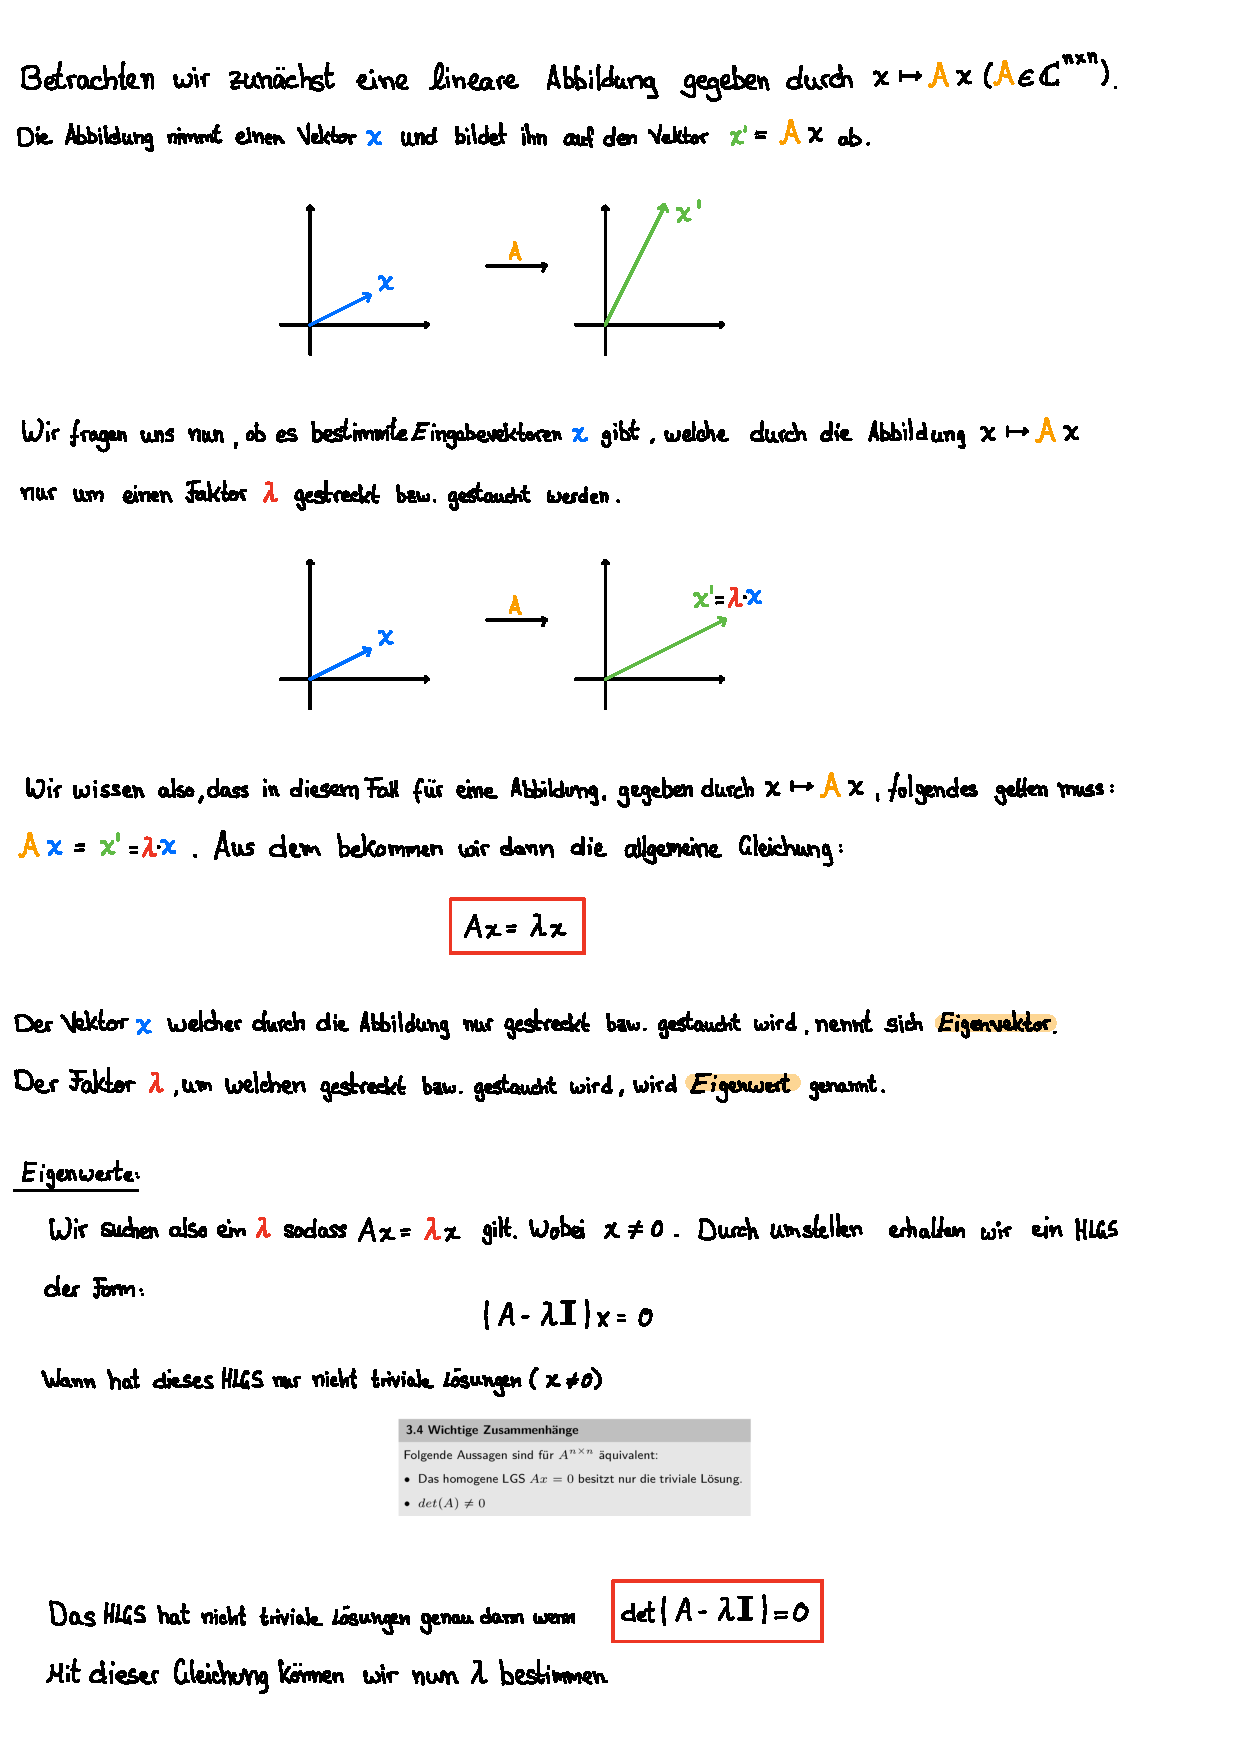
\includegraphics[page=1, scale=0.842]{pdf/06_Eigenwertproblem.pdf}
\end{figure}
\newpage
\includepdf[pages={2-}, 
            pagecommand={\thispagestyle{plain}}, 
            scale=0.95]{pdf/06_Eigenwertproblem.pdf}

\newgeometry{top=2.5cm, bottom=2cm}

\subsection{Beispielaufgaben} 

\vspace{1cm}

\subsubsection{} %Zardini S.93

Sei 

\begin{equation*}
    A = \begin{pmatrix}
    -3 & 4 & -4 \\
    0 & 5 & -8 \\
    0 & 4 & -7 \\
    \end{pmatrix}.
\end{equation*}

Bestimmen Sie die Eigenwerte und Eigenvektoren von \( A \) und geben Sie die geometrischen und algebraischen Vielfachheiten an. \\

\vspace{1\baselineskip}

\begin{solution}    

    \vspace{1\baselineskip}

    \leftskip=2em

    Eigenwerte durch det\( (A - \lambda \mathbb{I}) = 0 \) bestimmen. 

    \begin{equation*}
        \begin{aligned}
            \rightarrow & \begin{vmatrix}
                -3 - \lambda & 4 & -4 \\
                0 & 5 - \lambda & -8 \\
                0 & 4 & -7 - \lambda \\
            \end{vmatrix} = (-3 - \lambda) \begin{vmatrix}
                5 - \lambda & -8 \\
                4 & -7 - \lambda \\
                \end{vmatrix} \\[0.5em]
                &= \underbrace{(-3 - \lambda)}_{\lambda_1 = -3} \left[(5 - \lambda)(-7 - \lambda) + 32\right] = 0 \\[0.5em]
                \rightarrow & (5 - \lambda)(-7 - \lambda) + 32 = \lambda^2 + 2\lambda - 3 = \underbrace{(\lambda +3)}_{\lambda_2 = -3}\underbrace{(\lambda -1)}_{\lambda_3 = 1} = 0 
        \end{aligned}
    \end{equation*}

    Die Eigenwerte sind also \( \underbrace{\lambda_{1,2} = -3}_{\text{alg. vfh. 2}} \), und \( \underbrace{\lambda_3 = 1}_{\text{alg. vfh. 1}} \).

    \vspace{1\baselineskip}

    Nun die Eigenvektoren 

    \vspace{0.5\baselineskip}

    \( \rightarrow E_{-3}: \)
    \begin{equation*}
        \begin{gmatrix}[L]
            0 & 4 & -4 \\
            0 & 8 & -8 \\
            0 & 4 & -4 
        \end{gmatrix} \hspace{-0.75em} \begin{gmatrix}[R]
            0 \\ 0 \\ 0
        \end{gmatrix} \; \rightarrow \; \begin{gmatrix}[L]
            0 & 1 & -1 \\
            0 & 0 & 0 \\
            0 & 0 & 0
        \end{gmatrix} \hspace{-0.75em} \begin{gmatrix}[R]
            0 \\ 0 \\ 0
        \end{gmatrix} \; \rightarrow \; \begin{aligned}
            x_3 &= t \\
            x_2 &= s \\
            x_1 &= s
        \end{aligned} \qquad E_{-3} = \text{span} \left\{ \begin{pmatrix}
            1 \\ 0 \\ 0
        \end{pmatrix}, \begin{pmatrix}
            0 \\ 1 \\ 1
        \end{pmatrix} \right\} 
    \end{equation*}

    Die geometrische Vielfachheit von \( \lambda_{1,2} \) ist 2. 

    \vspace{1\baselineskip}

    \( \rightarrow E_{1}: \)
    \begin{equation*}
        \begin{gmatrix}[L]
            -4 & 4 & -4 \\
            0 & 4 & -8 \\
            0 & 4 & -8 
        \end{gmatrix} \hspace{-0.75em} \begin{gmatrix}[R]
            0 \\ 0 \\ 0
        \end{gmatrix} \; \rightarrow \; \begin{gmatrix}[L]
            -1 & 1 & -1 \\
            0 & 1 & -2 \\
            0 & 0 & 0 
        \end{gmatrix} \hspace{-0.75em} \begin{gmatrix}[R]
            0 \\ 0 \\ 0
        \end{gmatrix} \; \rightarrow \; \begin{aligned}
            x_3 &= t \\
            x_2 &= 2t \\
            x_1 &= 2t - t
        \end{aligned} \qquad E_{1} = \text{span} \left\{ \begin{pmatrix}
            1 \\ 2 \\ 1
        \end{pmatrix} \right\}
    \end{equation*}

    Die geometrische Vielfachheit von \( \lambda_{3} \) ist 1.

\end{solution}

\newpage

\subsubsection{} %Zardini S.96

Sei 

\begin{equation*}
    A = \begin{pmatrix}
    -3 & 4 & -4 \\
    0 & 5 & -8 \\
    0 & 4 & -7 \\
    \end{pmatrix}.
\end{equation*}

\begin{enumerate}[label=\alph*)]
    \item Berechnen Sie das charakteristische Polynom von \( A \) und überprüfen Sie ob \( A \) diagonalisierbar ist.
    \item Falls möglich, diagonalisieren Sie \( A \), sodass \[ D = T^{-1}AT\]
    \item Kann \( T \) orthogonal gewählt werden? Falls ja, geben Sie ein solches \( T \) an.
\end{enumerate}

\vspace{1\baselineskip}

\begin{solution}    

    \vspace{1\baselineskip}

    \leftskip=2em

    \textbf{a)} Aus 6.6.1 kennen wir bereits das charakteristische Polynom \[ p_A(\lambda) = (-3 - \lambda) \left[ (5 - \lambda)(-7 - \lambda) + 32 \right] = - (\lambda + 3)^2(\lambda - 1). \] Wir sahen auch, dass für jeden Eigenwert geom. Vfh. = alg. Vfh. gilt. Die Matrix ist also halbeinfach und deswegen Diagonalisierbar.

    \vspace{1\baselineskip}

    \textbf{b)} Mit den Eigenwerten und Eigenvektoren aus 6.6.1 können wir auch schnell \( D \) unf \( T \) aufschreiben. 

    \begin{equation*}
        D = \begin{pmatrix}
        -3 & 0 & 0 \\
        0 & -3 & 0 \\
        0 & 0 & 1 
        \end{pmatrix} \quad \text{und} \quad T = \begin{pmatrix}
            1 & 0 & 1 \\
            0 & 1 & 2 \\
            0 & 1 & 1 \\
        \end{pmatrix}
    \end{equation*}

    \vspace{1\baselineskip}

    \textbf{c)} \( T \) kann nicht orthogonal gewählt werden, da \( A \) nicht symmetrisch ist.

\end{solution}

\newpage

\subsubsection{} %Zardini S. 107

Sei \[ A = \begin{pmatrix} 5 & -6 \\ 3 & -4 \\ \end{pmatrix}. \] Berechnen Sie \( e^A \).

\vspace{1\baselineskip}

\textit{Tipp}: Das Matrixexponential vereinfacht sich für diagonalisierbare Matrizen als 
\[e^A = \sum_{n=0}^{\infty} \frac{A^n}{n!} = Tdiag(e^{\lambda_1}, ..., e^{\lambda_n})T^{-1}.\]

\vspace{1\baselineskip}

\begin{solution}    

    \vspace{1\baselineskip}

    \leftskip=2em

    Wir diagonalisieren \( A \) und berechnen dann \( e^A \) mit der Formel aus der Aufgabenstellung.

    \vspace{1\baselineskip}

    Eigenwerte:

    \begin{equation*}
        \begin{vmatrix}
            5 - \lambda & -6 \\
            3 & -4 - \lambda \\
        \end{vmatrix} = (5 - \lambda)(-4 - \lambda) + 18 = \lambda^2 - \lambda - 2 = (\lambda - 2)(\lambda + 1) = 0
    \end{equation*}

    \begin{equation*}
        \lambda_1 = -1, \quad \lambda_2 = 2
    \end{equation*}

    Eigenvektoren:

    \vspace{0.5\baselineskip}

    \( \rightarrow E_{-1} \):
    \begin{equation*}
        \begin{gmatrix}[L]
            6 & -6 \\
            3 & -3 
        \end{gmatrix} \hspace{-0.75em} \begin{gmatrix}[R]
            0 \\ 0
        \end{gmatrix} \; \rightarrow \; \begin{gmatrix}[L]
            1 & -1 \\
            0 & 0 
        \end{gmatrix} \hspace{-0.75em} \begin{gmatrix}[R]
            0 \\ 0
        \end{gmatrix} \; \rightarrow \; \begin{aligned}
            x_2 &= t \\
            x_1 &= t
        \end{aligned}  
        \qquad E_{-1} = \text{span} \left\{ \begin{pmatrix}
            1 \\ 1
        \end{pmatrix} \right\}
    \end{equation*}

    \( \rightarrow E_{2} \):
    \begin{equation*}
        \begin{gmatrix}[L]
            3 & -6 \\
            3 & -6 
        \end{gmatrix} \hspace{-0.75em} \begin{gmatrix}[R]
            0 \\ 0
        \end{gmatrix} \; \rightarrow \; \begin{gmatrix}[L]
            1 & -2 \\
            0 & 0 
        \end{gmatrix} \hspace{-0.75em} \begin{gmatrix}[R]
            0 \\ 0
        \end{gmatrix} \; \rightarrow \; \begin{aligned}
            x_2 &= t \\
            x_1 &= 2t
        \end{aligned}  
        \qquad E_{2} = \text{span} \left\{ \begin{pmatrix}
            2 \\ 1
        \end{pmatrix} \right\}
    \end{equation*}

    \begin{equation*}
        T = \begin{pmatrix}
            1 & 2 \\
            1 & 1
        \end{pmatrix}, \quad T^{-1} = \begin{pmatrix}
            -1 & 2 \\
            1 & -1
        \end{pmatrix}
    \end{equation*}

    Das Matrixexponential ist also

    \begin{equation*}
        e^A = \begin{pmatrix}
            1 & 2 \\
            1 & 1
        \end{pmatrix} \begin{pmatrix}
            e^{-1} & 0 \\
            0 & e^{2}
        \end{pmatrix} \begin{pmatrix}
            -1 & 2 \\
            1 & -1
        \end{pmatrix} = \begin{pmatrix}
            -e^{-1} + 2e^{2} & 2e^{-1} - 2e^{2} \\
            -e^{-1} + e^{2} & 2e^{-1} - e^{2}
        \end{pmatrix}
    \end{equation*}

\end{solution}

\newpage

\subsubsection{} %Zardini S. 110

Sei die quadratische Form \( q \) gegeben durch \[ \begin{aligned} q: \; \mathbb{R}^2 &\rightarrow \mathbb{R} \\ q(x) &\mapsto \frac{1}{2}x_1^2 + \sqrt{3}x_1x_2-\frac{1}{2}x_2^2 \;, \;x= \begin{pmatrix} x_1 \\ x_2\\ \end{pmatrix} \end{aligned} \]

\begin{enumerate}[label=\alph*)]
    \item Bestimmen Sie eine symmetrische Matrix \( A \), sodass \( q(x)=x^\top Ax \).
    \item Führen Sie die Hauptachsentransformation \( y=Tx \) durch und geben Sie die Normalform von \( q \) an.
\end{enumerate}

\vspace{1\baselineskip}

\begin{solution}    

    \vspace{1\baselineskip}

    \leftskip=2em

    \textbf{a)} \( A = \begin{pmatrix} \frac{1}{2} & \frac{\sqrt{3}}{2} \\ \frac{\sqrt{3}}{2} & -\frac{1}{2} \end{pmatrix} \)

    \vspace{1\baselineskip}

    \textbf{b)} Diagonalisieren:

    \begin{equation*}
        \begin{vmatrix}
            \frac{1}{2} - \lambda & \frac{\sqrt{3}}{2} \\
            \frac{\sqrt{3}}{2} & -\frac{1}{2} - \lambda
        \end{vmatrix} = \left(\frac{1}{2} - \lambda\right)\left(-\frac{1}{2} - \lambda\right) - \frac{3}{4} = \lambda^2 - 1 = 0 
    \end{equation*}

    \begin{equation*}
        \lambda_1 = -1, \quad \lambda_2 = 1
    \end{equation*}

    \begin{equation*}
        E_1: \begin{vmatrix}
            - \frac{1}{2} & \frac{\sqrt{3}}{2} \\
            \frac{\sqrt{3}}{2} & -\frac{3}{2}
        \end{vmatrix} \; \rightarrow \; E_1 = \text{span} \left\{ \begin{pmatrix}
            \sqrt{3} \\ 1
        \end{pmatrix} \right\}
    \end{equation*}

    \begin{equation*}
        E_{-1}: \begin{vmatrix}
            \frac{3}{2} & \frac{\sqrt{3}}{2} \\
            \frac{\sqrt{3}}{2} & \frac{1}{2}
        \end{vmatrix} \; \rightarrow \; E_{-1} = \text{span} \left\{ \begin{pmatrix}
            \frac{\sqrt{3}}{3} \\ -1
        \end{pmatrix} \right\}
    \end{equation*}

    Damit \( T \) orthogonal ist, müssen wir noch die Eigenvektoren normieren um dann \( T \) und \( D \) aufschreiben zu können. 

    \begin{equation*}
        T = \begin{pmatrix}
            \frac{\sqrt{3}}{2} & \frac{1}{2} \\
            \frac{1}{2} & -\frac{\sqrt{3}}{2} 
            \end{pmatrix}, \quad D = \begin{pmatrix}
                1 & 0 \\
                0 & -1
            \end{pmatrix}
    \end{equation*}

    Nun können wir die Hauptachsentransformation \( y = Tx \) durchführen.

    \begin{equation*}
        x^\top Ax \xrightarrow{x=T^{-1}y} (T^{-1}y)^\top A T^{-1}y = y^\top \underbrace{T A T^{-1}}_{D} y
    \end{equation*}

    \begin{equation*}
        \begin{pmatrix}
            y_1 & y_2
        \end{pmatrix} \begin{pmatrix}
            1 & 0 \\
            0 & -1
        \end{pmatrix} \begin{pmatrix}
            y_1 \\ y_2
        \end{pmatrix} = y_1^2 - y_2^2
    \end{equation*}

    \vspace{0.5\baselineskip}

    \begin{equation*}
        q(y) = y_1^2 - y_2^2
    \end{equation*}

\end{solution}
    \newgeometry{top=1cm, bottom=2cm}
\section{Methode der kleinsten Quadrate}
\begin{figure}[h!]
    \includegraphics[page=1, scale=0.842]{pdf/07_Methode_der_kleinsten_Quarate.pdf}
\end{figure}
\newpage
\includepdf[pages={2-}, 
            pagecommand={\thispagestyle{plain}}, 
            scale=0.95]{pdf/07_Methode_der_kleinsten_Quarate.pdf}

\newgeometry{top=2.5cm, bottom=2cm}

\subsection{Beispielaufgaben} 

\vspace{1cm}

\subsubsection{} %Übung 09

Sei 

\begin{equation*}
    \begin{aligned}
        &x_1 +& 0&x_2 =& 2\\
        &x_1 +&  &x_2 =& 1\\
        &x_1 +& 2&x_2 =& 0\\
        &x_1 +& 3&x_2 =& -1\\
        &x_1 +& 4&x_2 =& 1 
    \end{aligned}
\end{equation*}

ein überbestimmtes lineares Gleichungssystem. Lösen Sie das Ausgleichproblem mittels der Methode der kleinsten Quadrate. Das heisst, finden Sie \( (\hat{x}_1,\hat{x}_2)^\top \), so dass \( \|r\|_2 = \|Ax-c\|_2 \) minimal ist.

\vspace{1\baselineskip}

\begin{solution}    

    \vspace{1\baselineskip}

    \leftskip=2em

    \begin{equation*}
        A = \begin{pmatrix}
            1 & 0\\
            1 & 1\\
            1 & 2\\
            1 & 3\\
            1 & 4
        \end{pmatrix}, \quad
        c = \begin{pmatrix}
            2\\
            1\\
            0\\
            -1\\
            1
        \end{pmatrix}
    \end{equation*}

    \vspace{1\baselineskip}

    \begin{equation*}
        A^\top A = \begin{pmatrix}
            1 & 1 & 1 & 1 & 1\\
            0 & 1 & 2 & 3 & 4
        \end{pmatrix} \begin{pmatrix}
            1 & 0\\
            1 & 1\\
            1 & 2\\
            1 & 3\\
            1 & 4
        \end{pmatrix} = \begin{pmatrix}
            5 & 10\\
            10 & 30
        \end{pmatrix}
    \end{equation*}

    \vspace{1\baselineskip}

    \begin{equation*}
        A^\top c = \begin{pmatrix}
            1 & 1 & 1 & 1 & 1\\
            0 & 1 & 2 & 3 & 4
        \end{pmatrix} \begin{pmatrix}
            2\\
            1\\
            0\\
            -1\\
            1
        \end{pmatrix} = \begin{pmatrix}
            3\\
            2
        \end{pmatrix}
    \end{equation*}

    Löse \( A^\top A \hat{x} = A^\top c \):

    \begin{equation*}
        \begin{gmatrix}[L]
            5 & 10 \\
            10 & 30
        \end{gmatrix} \hspace{-0.75em} \begin{gmatrix}[R]
            3 \\ 2
                \rowops
                    \add[-2]{0}{1}
        \end{gmatrix} \; \rightarrow \;
        \begin{gmatrix}[L]
            5 & 10 \\
            0 & 10
        \end{gmatrix} \hspace{-0.75em} \begin{gmatrix}[R]
            3 \\ -4
        \end{gmatrix} \; \rightarrow \; \left\{ \begin{aligned}
            \hat{x}_2 &= - \frac{2}{5} \\[0.5em]
            \hat{x}_1 &= \frac{7}{5}
        \end{aligned} \right.
    \end{equation*}
        

\end{solution}

\newpage

\subsubsection{}

Gegeben sei

\begin{equation*}
    \begin{aligned}
        &x_1 +&  &x_2 &- 1 =&\; r_1\\
        &     &  &x_2 &- 3 =&\; r_2\\
        &     &  &x_2 &- 4 =&\; r_3\\
    \end{aligned}
\end{equation*}

Lösen Sie das Ausgleichsproblem mittels der QR-Zerlegung. 

\vspace{1\baselineskip}

\begin{solution}    

    \vspace{1\baselineskip}

    \leftskip=2em

    \begin{equation*}
        A = \begin{pmatrix}
            1 & 1\\
            0 & 1\\
            0 & \textcolor{red}{1}
        \end{pmatrix}, \quad
        c = \begin{pmatrix}
            1\\
            3\\
            4
        \end{pmatrix}
    \end{equation*}

    \vspace{1\baselineskip}

    Das Element \( a_{32} \) muss eleminiert werden, wir notieren also
    
    \begin{equation*}
        i = 3, \ i = 2, \ a_{22} = 1, \ a_{32} = 1, \ \omega = \sqrt{2}. 
    \end{equation*}

    Dadurch ist

    \begin{equation*}
        Q^{\top} = \begin{pmatrix}
            1 & 0 & 0\\
            0 & \cos \varphi & \sin \varphi\\
            0 & -\sin \varphi & \cos \varphi
        \end{pmatrix} \ \text{mit} \; \left\{ \begin{aligned}
            \cos \varphi &= \frac{1}{\sqrt{2}}\\
            \sin \varphi &= \frac{1}{\sqrt{2}}
        \end{aligned} \right.
    \end{equation*}

    \vspace{1\baselineskip}

    \begin{equation*}
        Q^\top A = \begin{pmatrix}
            1 & 0 & 0\\
            0 & \cos \varphi & \sin \varphi\\
            0 & -\sin \varphi & \cos \varphi
        \end{pmatrix} \begin{pmatrix}
            1 & 1\\
            0 & 1\\
            0 & 1
        \end{pmatrix} = \begin{pmatrix}
            1 & 1\\
            0 & \sqrt{2}\\
            0 & 0
        \end{pmatrix} \; \rightarrow \; R_0 = \begin{pmatrix}
            1 & 1\\
            0 & \sqrt{2}
        \end{pmatrix}
    \end{equation*}

    \vspace{1\baselineskip}

    \begin{equation*}
        Q^\top c = \begin{pmatrix}
            1 & 0 & 0\\
            0 & \cos \varphi & \sin \varphi\\
            0 & -\sin \varphi & \cos \varphi
        \end{pmatrix} \begin{pmatrix}
            1\\
            3\\
            4
        \end{pmatrix} = \begin{pmatrix}
            1\\
            \frac{7 \sqrt{2}}{2}\\
            \frac{\sqrt{2}}{2}
        \end{pmatrix}  \; \rightarrow \; d_0 = \begin{pmatrix}
            1\\
            \frac{7 \sqrt{2}}{2}
        \end{pmatrix}
    \end{equation*}

    Nun lösen wir das Gleichungssystem \( R_0 \hat{x} = d_0 \):

    \begin{equation*}
        \begin{gmatrix}[L]
            1 & 1 \\
            0 & \sqrt{2}
        \end{gmatrix} \hspace{-0.75em} \begin{gmatrix}[R]
            1 \\ \frac{7\sqrt{2}}{2}
        \end{gmatrix} \; \rightarrow \; \hat{x} = \begin{pmatrix}
            -\frac{5}{2} \\
            \frac{7}{2}
        \end{pmatrix} 
    \end{equation*}

\end{solution}
    \newgeometry{top=1cm, bottom=2cm}
\section{Lineare Differentialgleichungssysteme}
\begin{figure}[h!]
    \includegraphics[page=1, scale=0.842]{pdf/08_Lineare_diff_systeme.pdf}
\end{figure}
\newpage
\includepdf[pages={2-}, 
            pagecommand={\thispagestyle{plain}}, 
            scale=0.95]{pdf/08_Lineare_diff_systeme.pdf}

\newgeometry{top=2.5cm, bottom=2cm}

\subsection{Beispielaufgaben}

\vspace{1cm}

\subsubsection{} %Zardini S. 137

Sei \[ A = \begin{pmatrix} 1 & 1 \\ 6 & 2 \\ \end{pmatrix}. \] Lösen Sie das Anfangswertproblem \[ y'=Ay \;, \; y(0)= \begin{pmatrix} 0 \\ 10 \\ \end{pmatrix} \]

\vspace{1\baselineskip}

\begin{solution}    

    \leftskip=2em

    \begin{equation*}
        \begin{vmatrix}
            1-\lambda & 1\\
            6 & 2-\lambda
        \end{vmatrix} = (1-\lambda)(2-\lambda) - 6 = \lambda^2 - 3\lambda - 4 = (\lambda-4)(\lambda+1) = 0
    \end{equation*}

    \begin{equation*}
        \lambda_1 = 4, \quad \lambda_2 = -1
    \end{equation*}

    \( E_4: \)

    \begin{equation*}
        \begin{gmatrix}[L]
            -3 & 1\\
            6 & -2
        \end{gmatrix} \hspace{-0.75em} \begin{gmatrix}[R]
            0\\
            0
        \end{gmatrix} \rightarrow \begin{gmatrix}[L]
            -3 & 1\\
            0 & 0
        \end{gmatrix} \hspace{-0.75em} \begin{gmatrix}[R]
            0\\
            0
        \end{gmatrix} \; \rightarrow \; \left\{ \begin{aligned}
            x_2 &= t \\
            x_1 &= \frac{t}{3}
            \end{aligned} 
        \right. \qquad E_4 = \text{span} \left\{ \begin{pmatrix} 1 \\ 3 \end{pmatrix} \right\}
    \end{equation*}

    \( E_{-1}: \)
    \begin{equation*}
        \begin{gmatrix}[L]
            2 & 1\\
            6 & 3
        \end{gmatrix} \hspace{-0.75em} \begin{gmatrix}[R]
            0\\
            0
        \end{gmatrix} \rightarrow \begin{gmatrix}[L]
            2 & 1\\
            0 & 0
        \end{gmatrix} \hspace{-0.75em} \begin{gmatrix}[R]
            0\\
            0
        \end{gmatrix} \; \rightarrow \; \left\{ \begin{aligned}
            x_2 &= t\\
            x_1 &= -\frac{t}{2}
            \end{aligned} 
        \right. \qquad E_{-1} = \text{span} \left\{ \begin{pmatrix} 1 \\ -2 \end{pmatrix} \right\}
    \end{equation*}

    Die allgemeine Lösung ist also

    \begin{equation*}
        y(t) = c_1 \begin{pmatrix} 1 \\ 3 \end{pmatrix} e^{4t} + c_2 \begin{pmatrix} 1 \\ -2 \end{pmatrix} e^{-t}
    \end{equation*}

    Nun fehlt noch die Anfangsbedingung

    \begin{equation*}
        y(0) = c_1 \begin{pmatrix} 1 \\ 3 \end{pmatrix} + c_2 \begin{pmatrix} 1 \\ -2 \end{pmatrix} = \begin{pmatrix} 0 \\ 10 \end{pmatrix} \rightarrow \; \begin{gmatrix}[L]
            1 & 1\\
            3 & -2
        \end{gmatrix} \hspace{-0.75em} \begin{gmatrix}[R]
            0\\
            10
        \end{gmatrix} \; \rightarrow \; c_1 = -c_2 = 2
    \end{equation*}

    Damit ist die Lösung des Anfangswertproblems

    \begin{equation*}
        y(t) = 2 \begin{pmatrix} 1 \\ 3 \end{pmatrix} e^{4t} - 2 \begin{pmatrix} 1 \\ -2 \end{pmatrix} e^{-t} = \begin{pmatrix} 2e^{4t} - 2e^{-t} \\ 6e^{4t} + 4e^{-t} \end{pmatrix}
    \end{equation*}

\end{solution}

\newpage

\subsubsection{} %Übung 11 (S17)

Gegeben sei die Differentialgleichung 2. Ordnung

\begin{equation}
    x''(t) = -8x(t) + 4x'(t)  
    \tag{$\dagger$}
\end{equation}

\begin{enumerate}[label=\alph*)]
    \item Verwandeln Sie (\( \dagger \)) in ein Differentialgleichungssystem 1. Ordnung. Welche Dimension hat der Lösungsraum dieses Systems?
    \item Geben Sie die allgemeine reelle Lösung der Differentialgleichung (\( \dagger \)) an.
    \item Bestimmen Sie die Lösung von (\( \dagger \)) zu den Bedingungen \( x(0) = 1, x(\frac{\pi}{4})=1 \).
\end{enumerate}

\vspace{1\baselineskip}

\begin{solution}    

    \vspace{1\baselineskip}

    \leftskip=2em

    \textbf{a)} Zuerst wandeln wir (\( \dagger \)) in ein System 1. Ordnung um. Die Substitution

    \begin{equation*}
        \begin{aligned}
            y_0 &:= x \\
            y_1 &:= x' \\
            y_2 &:= x''         
        \end{aligned} \qquad \longrightarrow \qquad
        \begin{aligned}
            y_1 = y_0' \\
            y_2 = y_1' 
        \end{aligned}
    \end{equation*}   

    führt zu dem Differentialgleichungssystem
    
    \begin{equation*}
        \left\{ \begin{aligned}
            y_0' &= y_1 \\
            y_1' &= -8y_0 + 4y_1
        \end{aligned} \right. \qquad \text{bzw.} \qquad
        \begin{pmatrix}
            y_0' \\
            y_1'
        \end{pmatrix} =
        \underbrace{\begin{pmatrix}
            0 & 1 \\
            -8 & 4
        \end{pmatrix}}_{A}
        \begin{pmatrix}
            y_0 \\
            y_1
        \end{pmatrix}.
    \end{equation*}

    \textbf{b)} Allgemeine \textbf{reelle} Lösung finden. 

    \begin{equation*}
        \text{det} \begin{pmatrix}
            -\lambda & 1 \\
            -8 & 4 - \lambda
        \end{pmatrix} = \lambda^2 - 4\lambda + 8 = 0 \quad \rightarrow \quad
        \lambda_{1,2} = 2 \pm 2i,
    \end{equation*}

    \begin{equation*}
        E_{2+2i} : \begin{gmatrix}[L]
            -2-2i & 1 \\
            -8 & 2-2i
        \end{gmatrix} \hspace{-0.75em}
        \begin{gmatrix}[R]
            0 \\ 0
            \rowops
            \add[\cdot\frac{-8}{2+2i}]{0}{1}
        \end{gmatrix} \rightarrow \quad
        \begin{gmatrix}[L]
            -2-2i & 1 \\
            0 & 0
        \end{gmatrix} \hspace{-0.75em}
        \begin{gmatrix}[R]
            0 \\ 0
        \end{gmatrix} \quad \left\{ \begin{aligned}
            y_0 &= \frac{s}{2+2i} \\[0.5em]
            y_1 &= s \in \mathbb{R} 
        \end{aligned} \right.
    \end{equation*}

    \vspace{1\baselineskip}

    \begin{equation*}
        \text{für} \ s = 4 \quad \left\{ \begin{aligned}
            y_0 &= \frac{4}{2+2i} \cdot \underbrace{\frac{2-2i}{2-2i}}_{=1} = \frac{4(2-2i)}{4+4} = 1-i \\
            y_1 &= 4 
        \end{aligned} \right.
    \end{equation*}

    \vspace{1\baselineskip}

    \begin{equation*}
        E_{2+2i} : \ \text{span} \left\{ \begin{pmatrix}
            1-i \\ 4
        \end{pmatrix} \right\} \ , \quad 
        E_{2-2i} : \ \text{span} \left\{ \begin{pmatrix}
            1+i \\ 4
        \end{pmatrix} \right\}.
    \end{equation*}

    Wodurch sich die folgende allgemeine Lösung des Systems ergibt

    \begin{equation*}
        y(t) = e^{(2+2i)t} \begin{pmatrix}
            1-i \\ 4
        \end{pmatrix} + e^{(2-2i)t} \begin{pmatrix}
            1+i \\ 4
        \end{pmatrix}.
    \end{equation*}

    Diese Lösung ist jedoch komplex. Normalerweise wollen wir aber eine reelle Lösung. Um eine reelle Lösung zu erhalten, benutzten wir die Eulersche Formel \( r e^{i \phi} = r \cos(\phi) + i \ r \sin(\phi) \). Um die Notation folgend zu vereinfachen betrachten, wir nur einen der beiden Eigenvektoren der Lösung (wenn man beide betrachtet kommt man auf das gleiche Ergebnis nur mit mehr Notation, am Ende findest du die Alternative mit beiden). 

    \begin{equation*}
        \begin{aligned}
            y(t) &= e^{(2+2i)t} \begin{pmatrix}
                1-i \\ 4
            \end{pmatrix} =
            e^{2t} e^{2it} \begin{pmatrix}
                1-i \\ 4
            \end{pmatrix} \\[0.5em]
            &= e^{2t} \left( \cos(2t) + i \sin(2t) \right) \begin{pmatrix}
                1-i \\ 4
            \end{pmatrix} \\[0.5em]
            &= e^{2t} \left\{ \begin{pmatrix}
                \cos(2t) + i \sin(2t) - i \cos(2t) - \sin(2t) \\
                4 \cos(2t) + 4i \sin(2t)
            \end{pmatrix} \right\} \\[0.5em]
            &= e^{2t} \left\{ \begin{pmatrix}
                \cos(2t) + \sin(2t) \\
                4 \cos(2t)
            \end{pmatrix} + i \begin{pmatrix}
                \sin(2t) - \cos(2t) \\
                4 \sin(2t)
            \end{pmatrix} \right\} 
        \end{aligned}
    \end{equation*}

    \vspace{0.5\baselineskip}

    Für den letzten Schritt benutzten wir ein Korollar aus der Vorlesung welches besagt, dass wenn \( y \) eine komplexe Lösung eines homogenen linearen Differentialgleichungssystems \( y'=Ay \) ist, so sind Re(\(y\)) und Im(\(y\)) ebenfalls Lösungen des Systems. Re(\(y\)) und Im(\(y\)) sind hier weiterhin linear unabhängig und bilden dadurch eine Basis des Lösungsraums von \( y \). So lässt sich eine allgemeine Lösung auch als Linearkombination von Re(\(y\)) und Im(\(y\)) schreiben

    \begin{equation*}
        y(t) = e^{2t} \left\{ a \begin{pmatrix}
            \cos(2t) + \sin(2t) \\
            4 \cos(2t)
        \end{pmatrix} + b \begin{pmatrix}
            \sin(2t) - \cos(2t) \\
            4 \sin(2t)
        \end{pmatrix} \right\}.
    \end{equation*}

    \vspace{0.5\baselineskip}

    Da wir eigentlich eine Lösung für \( (\dagger) \) suchen und durch die Substitution \( x = y_0 \) substituiert wurde, nehmen wir nur die erste Zeile des Vektors \( y(t) \). 

    \begin{equation*}
        \begin{aligned}
        x(t) = y_0(t) &= e^{2t} \left\{ a ( \cos(2t) + \sin(2t) ) + b ( \sin(2t) - \cos(2t) ) \right\} \\[0.5em]
        &= e^{2t} \left\{ (a-b) \cos(2t) + (a+b) \sin(2t) \right\} \\[0.5em]
        &= e^{2t} \left\{ c_1 \cos(2t) + c_2 \sin(2t) \right\}.
        \end{aligned}
    \end{equation*}

    \textbf{c)} Nun müssen wir die Anfangsbedingungen \( x(0) = 1 \) und \( x(\frac{\pi}{4})=1 \) in die allgemeine Lösung einsetzen.

    \begin{equation*}
        \begin{aligned}
            x(0) &= e^{2\cdot 0} \left\{ c_1 \cos(2\cdot 0) + c_2 \sin(2\cdot 0) \right\} = 1 \rightarrow c_1 = 1 \\[0.5em]
            x\left( \frac{\pi}{4} \right) &= e^{2\cdot \frac{\pi}{4}} \left\{ c_1 \cos\left( 2\cdot \frac{\pi}{4} \right) + c_2 \sin\left( 2\cdot \frac{\pi}{4} \right) \right\} = 1 \rightarrow c_2 = e^{-\frac{\pi}{2}}
        \end{aligned}
    \end{equation*}

    Damit ergibt sich die Lösung des Anfangswertproblems
    \begin{equation*}
        x(t) = e^{2t} \left\{ \cos(2t) + e^{-\frac{\pi}{2}} \sin(2t) \right\}.
    \end{equation*}

    \vspace{1\baselineskip}

    \textbf{Alternative Lösung mit beiden Eigenvektoren:}

    Anstatt nur einen der beiden Eigenvektoren zu benutzen, können wir auch beide benutzen. Das Resultat ist das gleiche, jedoch mit mehr Notationsaufwand.

    \begin{equation*}
        \begin{aligned}
            y(t) &= c_3 \cdot e^{(2+2i)t} \begin{pmatrix}
                1-i \\ 4
            \end{pmatrix} + c_4  \cdot e^{(2-2i)t} \begin{pmatrix}
                1+i \\ 4
            \end{pmatrix} \\[0.5em] 
            &= e^{2t} \left\{
                c_3 \left( 
                    \cos(2t) + i \sin(2t) \right) \begin{pmatrix}
                        1-i \\ 4
                    \end{pmatrix} + c_4  \left( 
                    \cos(2t) - i \sin(2t) \right) \begin{pmatrix}
                        1+i \\ 4
                    \end{pmatrix}
            \right\} \\[0.5em]
            &= e^{2t} \left( \text{\scriptsize $ \begin{matrix}
                c_3 \cos(2t) + c_3 i \sin(2t) - c_3 i \cos(2t) - c_3 \sin(2t) + c_4  \cos(2t) - c_4  i \sin(2t) + c_4  i \cos(2t) - c_4  \sin(2t) \\[0.5em]
                4 c_3 \cos(2t) + 4 c_3 i \sin(2t) + 4 c_4  \cos(2t) - 4 c_4  i \sin(2t)
            \end{matrix}$} \right) \\[0.5em]
            &= e^{2t} \left( \text{\scriptsize $ \begin{matrix}
                ( c_3 + c_4  ) \cos(2t) + ( c_3 - c_4  ) i \sin(2t) - ( c_3 - c_4  ) i \cos(2t) + ( c_3 + c_4  ) \sin(2t) \\
                4 ( c_3 + c_4  ) \cos(2t) + 4 ( c_3 - c_4  ) i \sin(2t)
            \end{matrix}$} \right) \\[0.5em]
            &= e^{2t} \left\{ \left( \text{\scriptsize $ \begin{gmatrix}[n]
                ( c_3 + c_4  ) \cos(2t) + ( c_3 + c_4  ) \sin(2t) \\
                4 ( c_3 + c_4  ) \cos(2t)
            \end{gmatrix} + i \begin{gmatrix}[m]   
                ( c_3 - c_4  ) \sin(2t) - ( c_3 - c_4  ) \cos(2t) \\
                4 ( c_3 - c_4  ) \sin(2t)
            \end{gmatrix}$} \right) \right\} \\[0.5em]
            &= e^{2t} \left\{ a \begin{pmatrix}
                \cos(2t) + \sin(2t) \\
                4 \cos(2t)
            \end{pmatrix} + i \ b \begin{pmatrix}
                \sin(2t) - \cos(2t) \\
                4 \sin(2t)
            \end{pmatrix} \right\} 
        \end{aligned}
    \end{equation*}

    womit wir schliesslich durch dieselbe Argumentation von oben die Lösung für \((\dagger)\) finden

    \begin{equation*}
        \begin{aligned}
        x(t) = y_0(t) &= e^{2t} \left\{ a ( \cos(2t) + \sin(2t) ) + b ( \sin(2t) - \cos(2t) ) \right\} \\[0.5em]
        &= e^{2t} \left\{ (a-b) \cos(2t) + (a+b) \sin(2t) \right\} \\[0.5em]
        &= e^{2t} \left\{ c_1 \cos(2t) + c_2 \sin(2t) \right\}.
        \end{aligned}
    \end{equation*}

\end{solution}

\newpage

\subsubsection{} %Zardini S. 154

Gegeben sei das Differentialgleichungssystem 2. Ordnung

\begin{equation*}
    \begin{aligned}
    y''(t) &= -2y(t) + z(t)\\
    z'(t) &= -6y(t) + 3z(t)
    \end{aligned}
\end{equation*}

\begin{enumerate}[label=\alph*)]
    \item Verwandeln Sie das Differentialgleichungssystem in ein System 1. Ordnung. 
    \item Geben Sie die allgemeine Lösung des in a) gefundenen Systems an.
\end{enumerate} 

\vspace{1\baselineskip}

\begin{solution}    

    \vspace{1\baselineskip}

    \leftskip=2em

    \textbf{a)} Substitution
    \begin{equation*}
        \begin{aligned}
            y' &:= x \\
            y'' &:= x' 
        \end{aligned} \quad \rightarrow \quad
        \begin{aligned}
            x' &= -2y + z \\
            y' &= x \\
            z' &= -6y + 3z
        \end{aligned} \quad \rightarrow \quad
        \begin{pmatrix}
            x' \\
            y' \\
            z'
        \end{pmatrix} =
        \begin{pmatrix}
            0 & -2 & 1 \\
            1 & 0 & 0 \\
            0 & -6 & 3
        \end{pmatrix}
        \begin{pmatrix}
            x \\
            y \\
            z
        \end{pmatrix}.
    \end{equation*}

    \textbf{b)} Allgemeine Lösung finden

    \vspace{1\baselineskip}

    Eigenwerte und Eigenvektoren ergeben:

    \begin{equation*}
        \lambda_1 = 0, \ \lambda_2 = 1, \ \lambda_3 = 2  
    \end{equation*}

    \begin{equation*}
        v_1 = \begin{pmatrix} 0 \\ 1 \\ 2 \end{pmatrix}, \ v_2 = \begin{pmatrix} 1 \\ 1 \\ 3 \end{pmatrix}, \ v_3 = \begin{pmatrix} 2 \\ 1 \\ 6 \end{pmatrix}.
    \end{equation*}

    \vspace{1\baselineskip}

    \begin{equation*}
        D = \begin{pmatrix}
            0 & 0 & 0 \\
            0 & 1 & 0 \\
            0 & 0 & 2
        \end{pmatrix}, \quad
        T = \begin{pmatrix}
            0 & 1 & 2 \\
            1 & 1 & 1 \\
            2 & 3 & 6
        \end{pmatrix}
    \end{equation*}

    \vspace{1\baselineskip}

    Die Allgemeine Lösung des Systems ist also

    \begin{equation*}
        \begin{pmatrix}
            x \\
            y \\
            z
        \end{pmatrix} = c_1 \begin{pmatrix} 0 \\ 1 \\ 2 \end{pmatrix} + c_2 e^{t} \begin{pmatrix} 1 \\ 1 \\ 3 \end{pmatrix} + c_3 e^{2t} \begin{pmatrix} 2 \\ 1 \\ 6 \end{pmatrix}
    \end{equation*}

\end{solution}
\end{document}
